%
% Mechanical.tex
% Mechanical Development
%
% LulzBot Mini Developer's Guide
%
% Copyright (C) 2014 Aleph Objects, Inc.
%
% This document is licensed under the Creative Commons Attribution 4.0
% International Public License (CC BY-SA 4.0) by Aleph Objects, Inc.
%

\section{Intro}
Mechanical hardware specs and parts are in these subdirectories:

\url{http://devel.lulzbot.com/mini/}

\section{Bill of Materials}

% pdfjam  --papersize '{24.58cm,18.90cm}'   --no-landscape daffodil_bom.pdf '1-3'
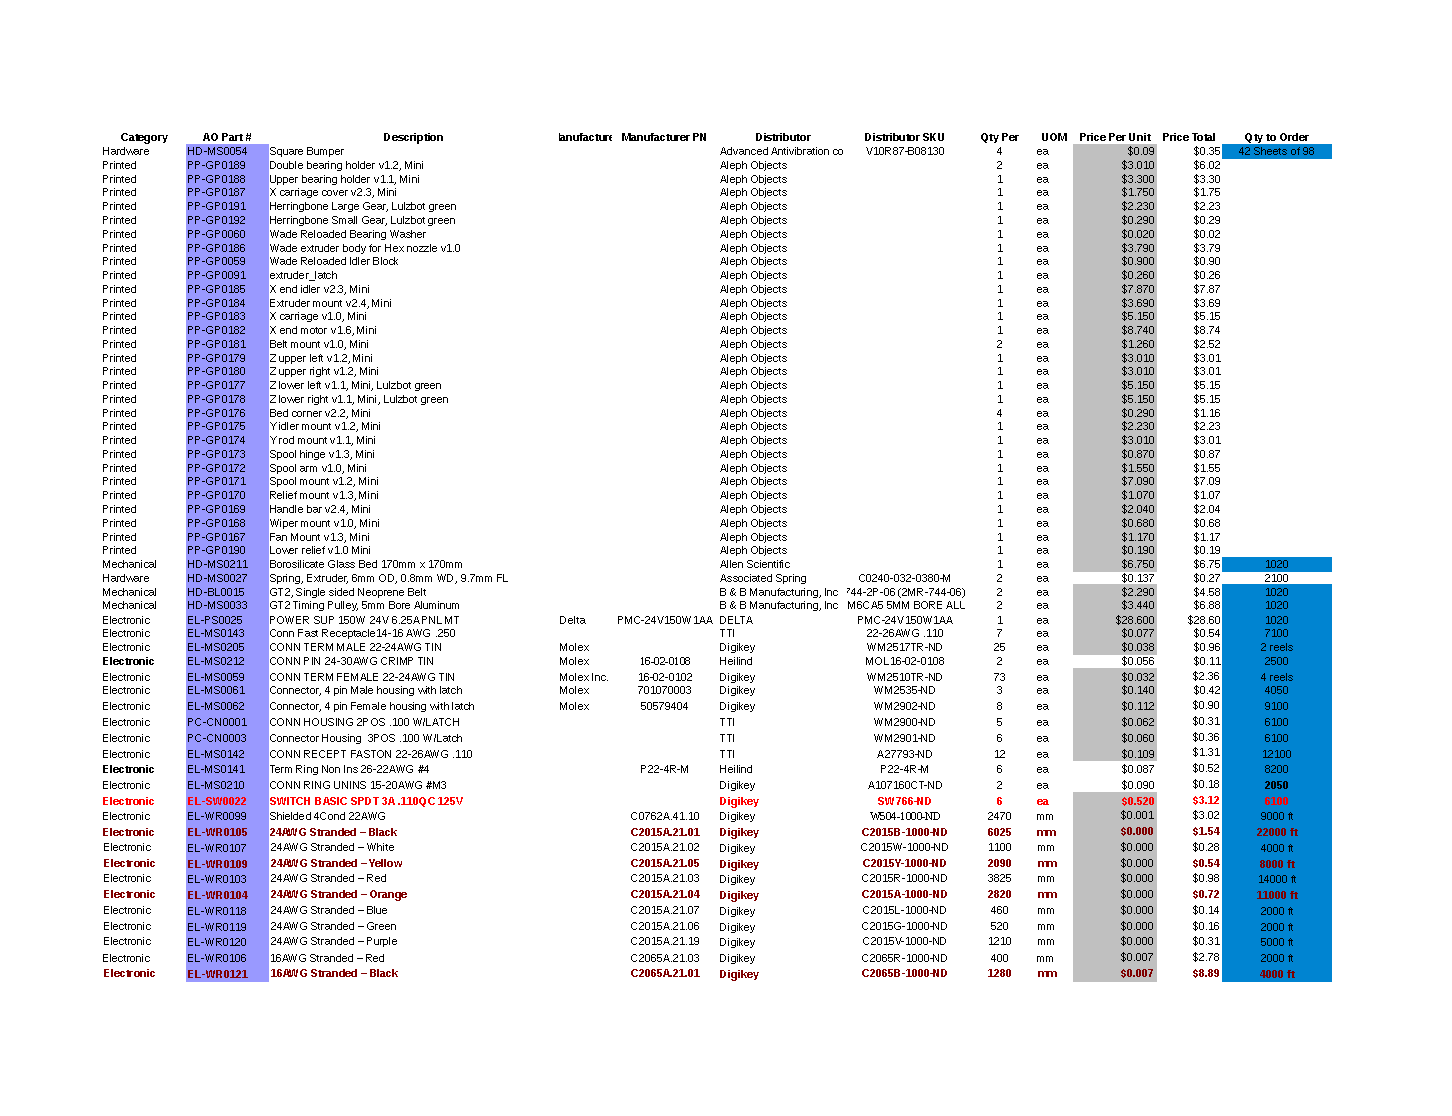
\includepdf[addtolist={1,figure,{Bill of Materials},bom},pages=-,landscape=true,reflect=false,turn=false,fitpaper=true,keepaspectratio=true]{bom.pdf}

\section{Drawings}
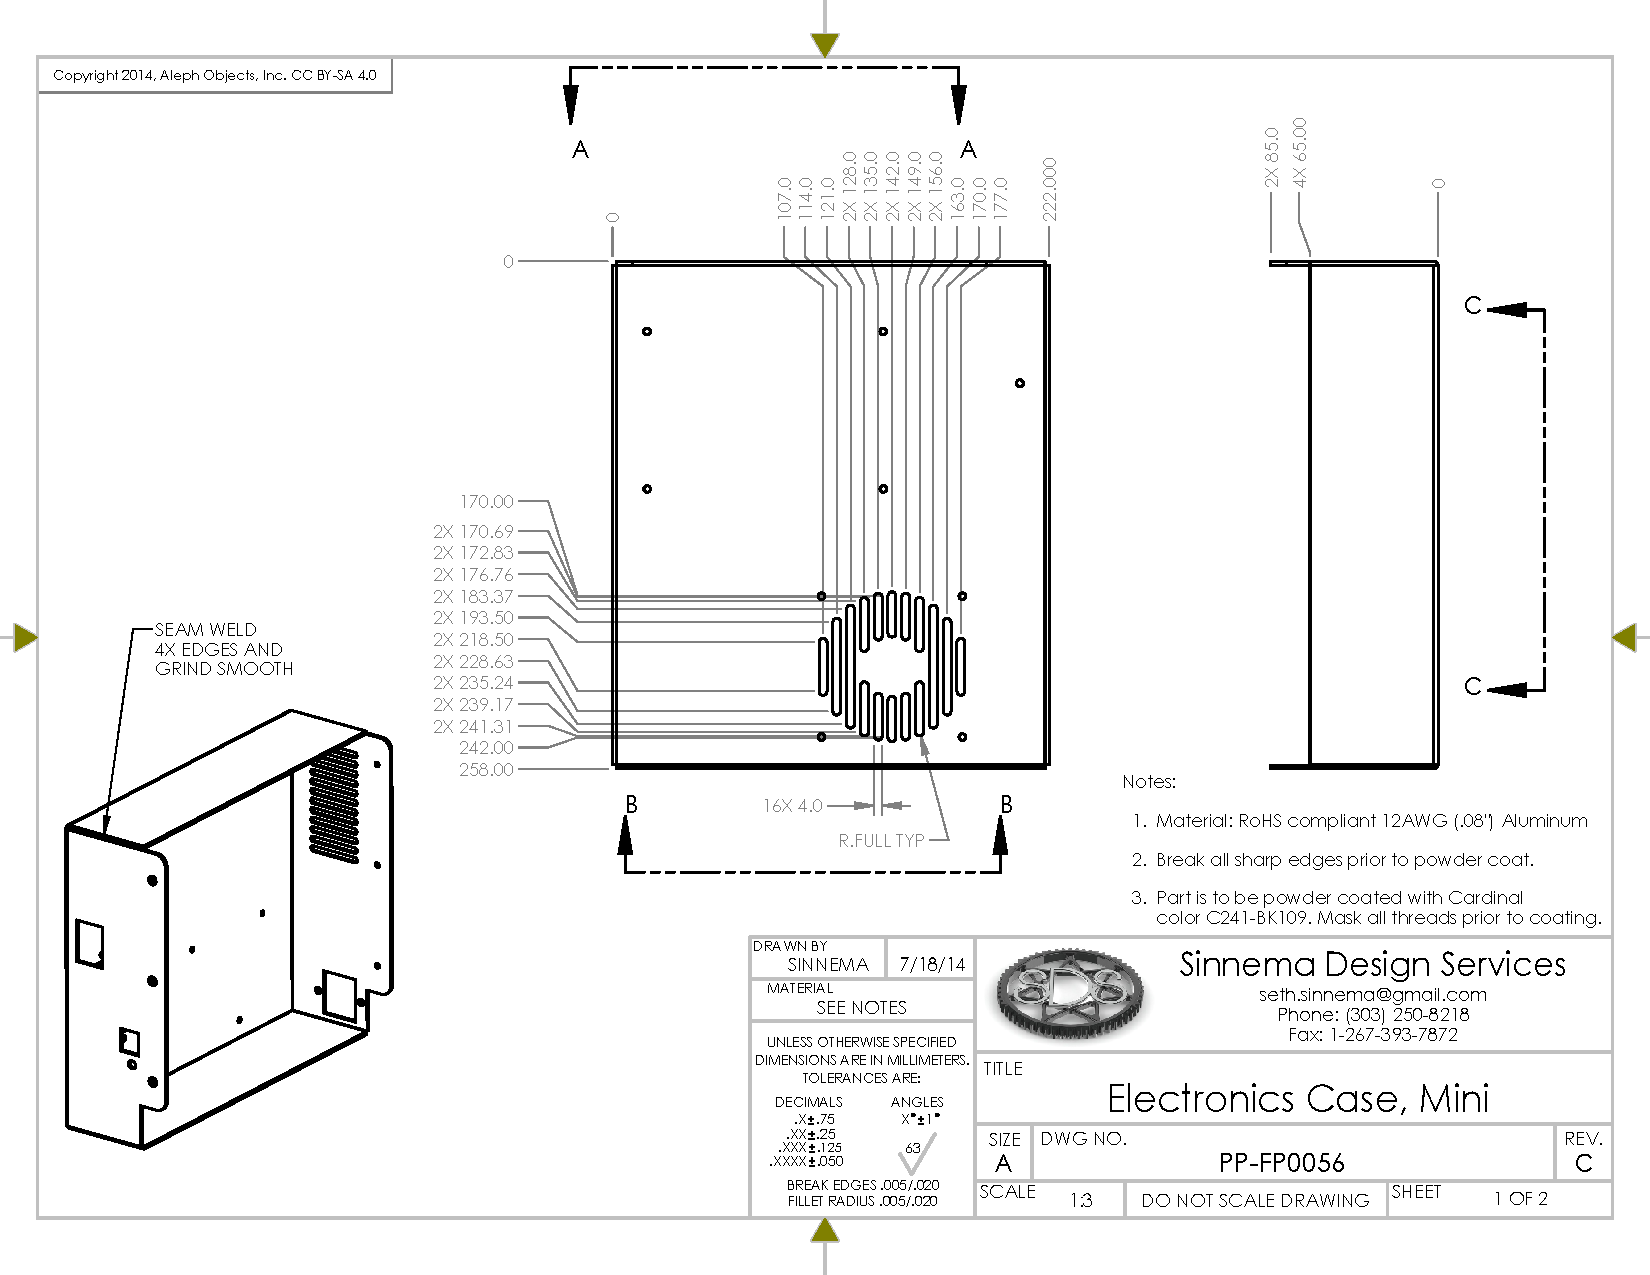
\includepdf[addtolist={1,figure,{Electronics Case},eleccase},pages=-,landscape=true,reflect=false,turn=false,fitpaper=true,keepaspectratio=true]{PP-FP0056rC.pdf}
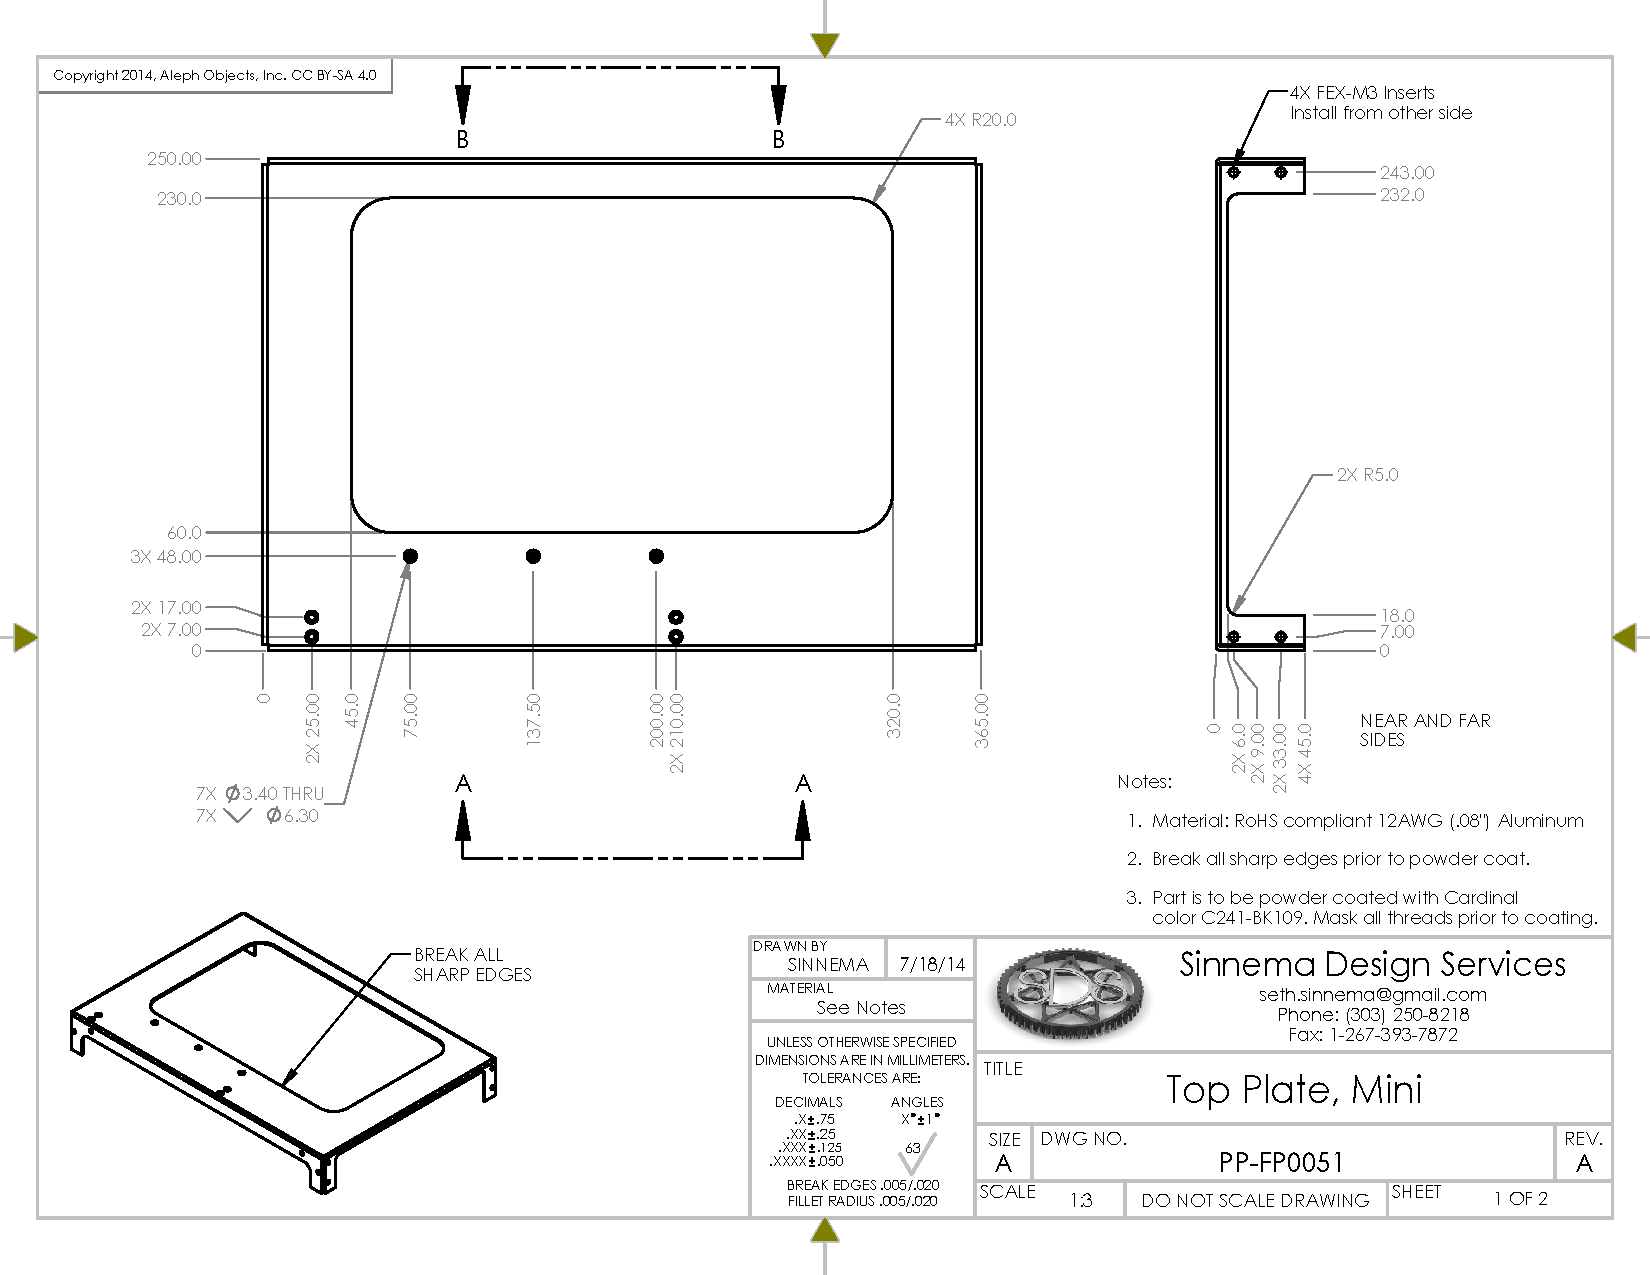
\includepdf[addtolist={1,figure,{Top Plate},topplate},pages=-,landscape=true,reflect=false,turn=false,fitpaper=true,keepaspectratio=true]{PP-FP0051rA.pdf}
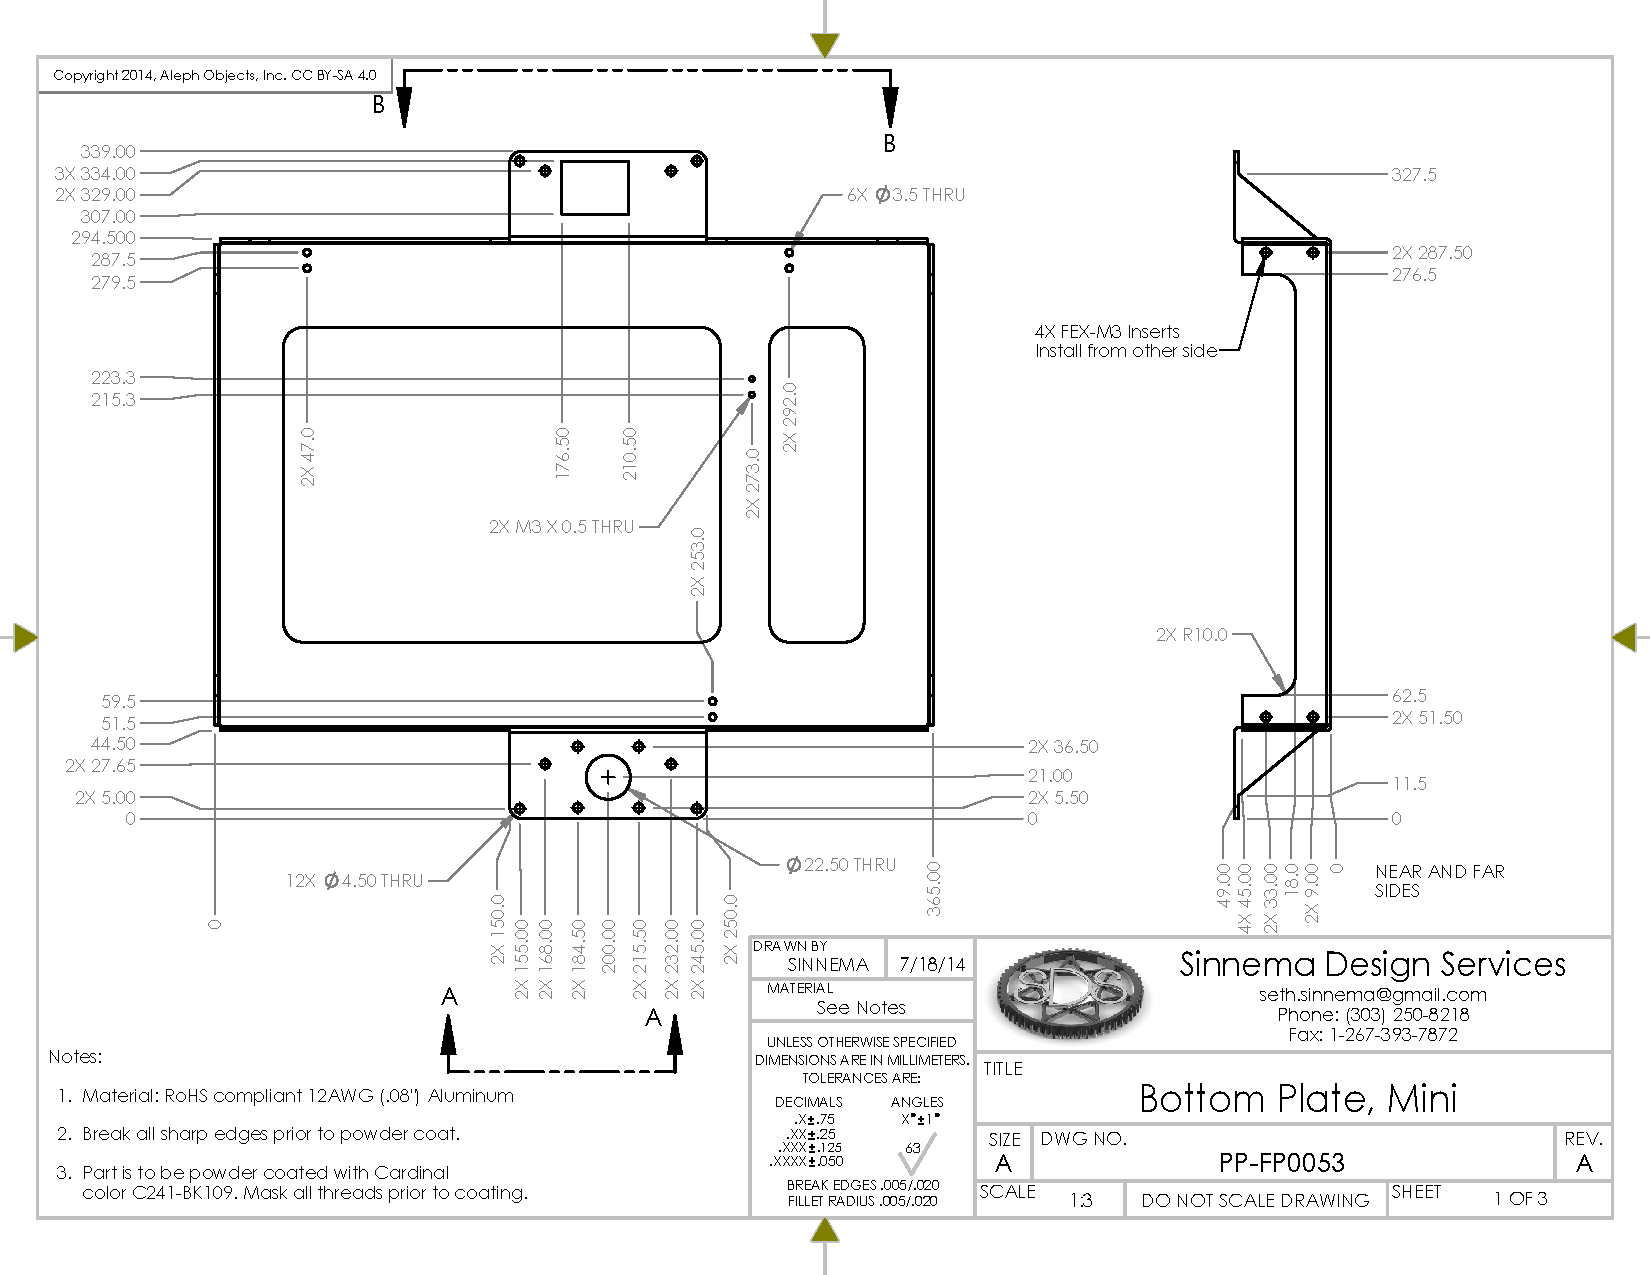
\includepdf[addtolist={1,figure,{Bottom Plate},bottomplate},pages=-,landscape=true,reflect=false,turn=false,fitpaper=true,keepaspectratio=true]{PP-FP0053rA.pdf}
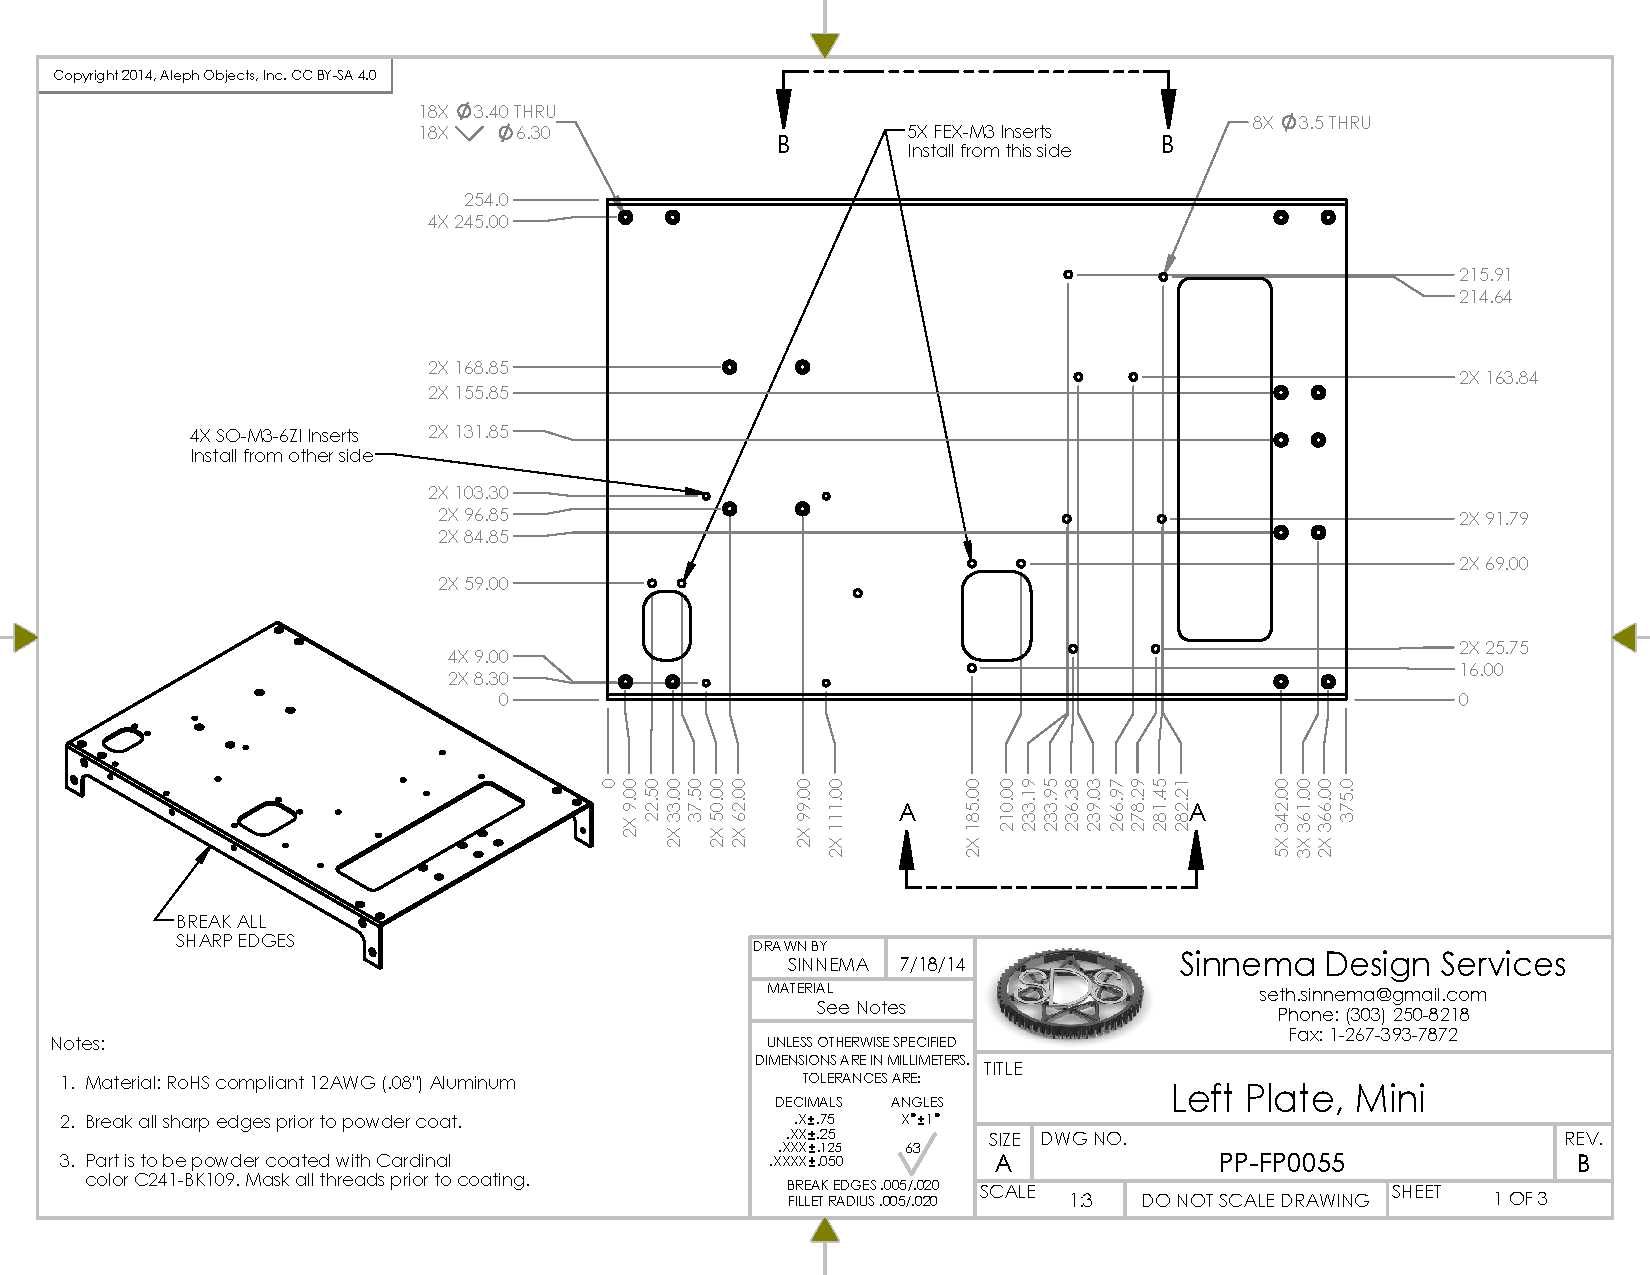
\includepdf[addtolist={1,figure,{Left Plate},leftplate},pages=-,landscape=true,reflect=false,turn=false,fitpaper=true,keepaspectratio=true]{PP-FP0055rB.pdf}
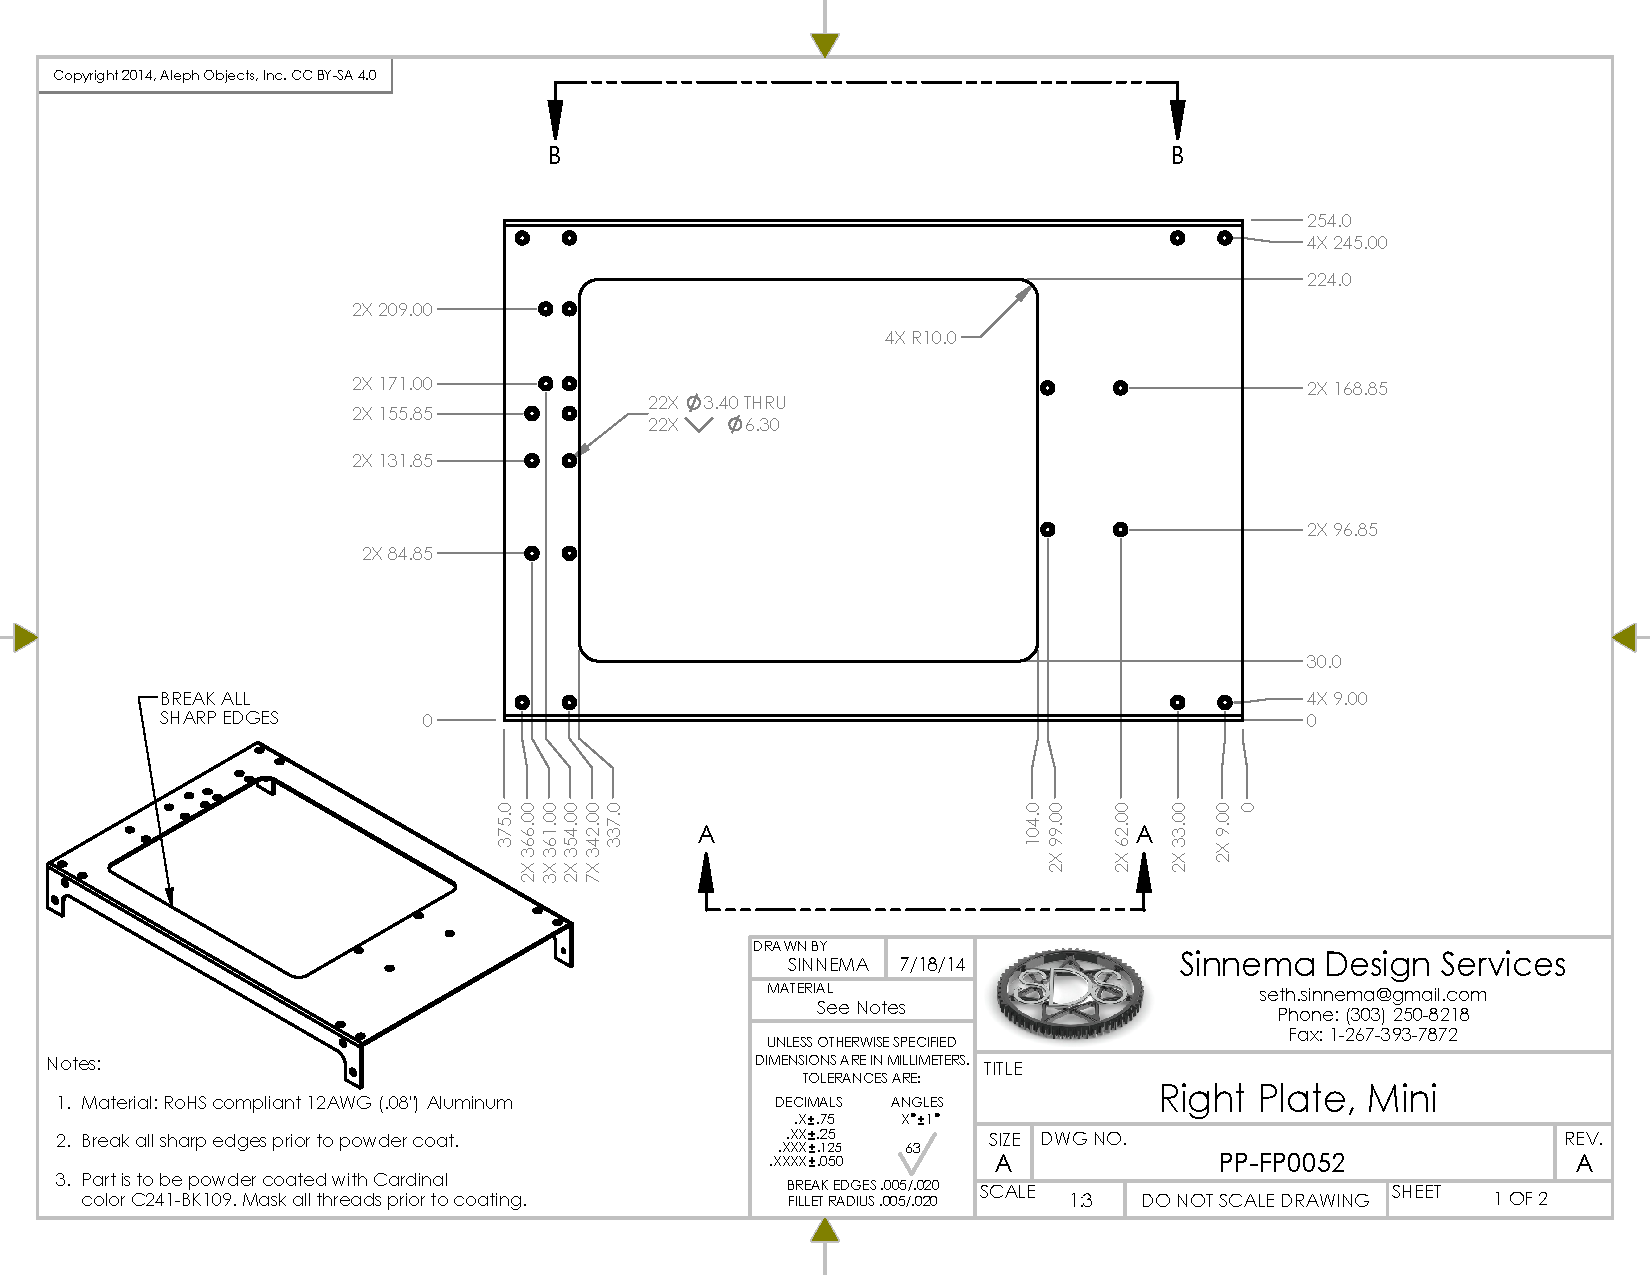
\includepdf[addtolist={1,figure,{Right Plate},rightplate},pages=-,landscape=true,reflect=false,turn=false,fitpaper=true,keepaspectratio=true]{PP-FP0052rA.pdf}
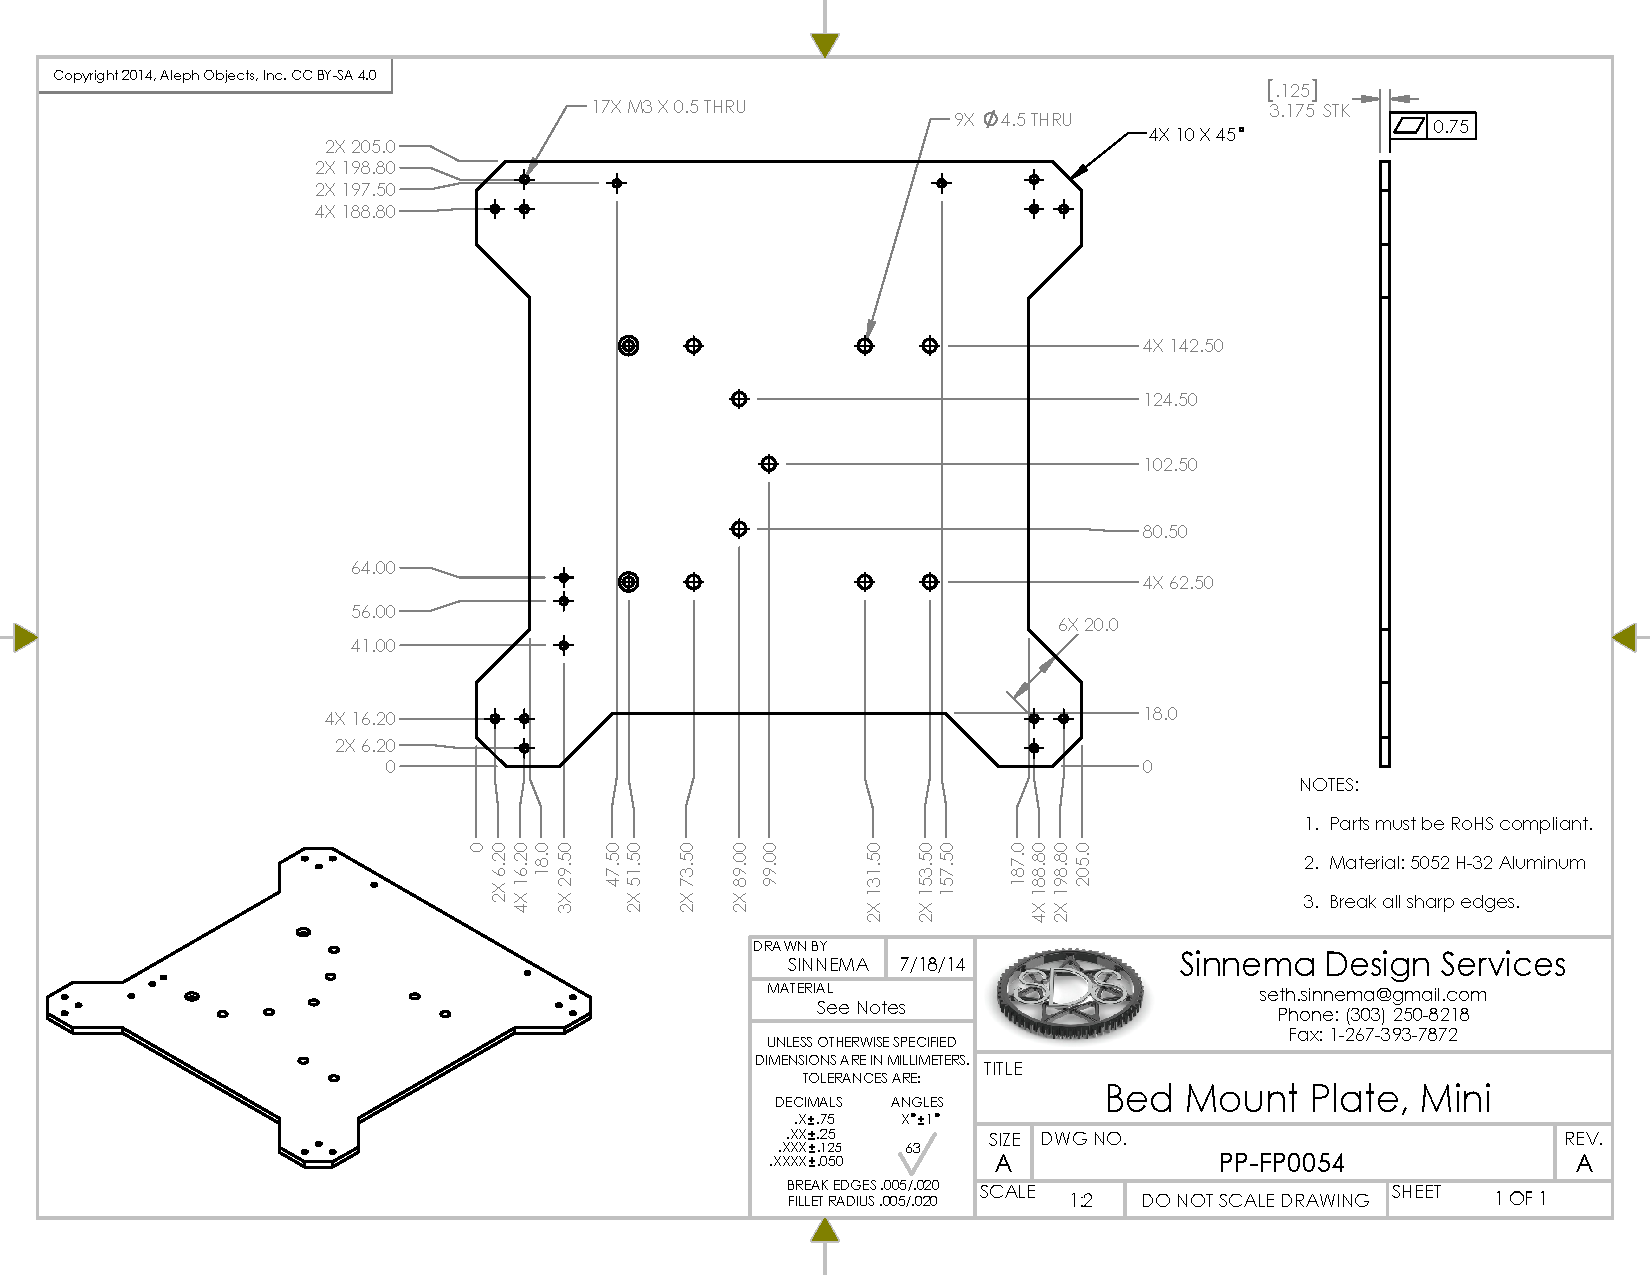
\includepdf[addtolist={1,figure,{Bed Mount Plate},bedmountplate},pages=-,landscape=true,reflect=false,turn=false,fitpaper=true,keepaspectratio=true]{PP-FP0054rA.pdf}
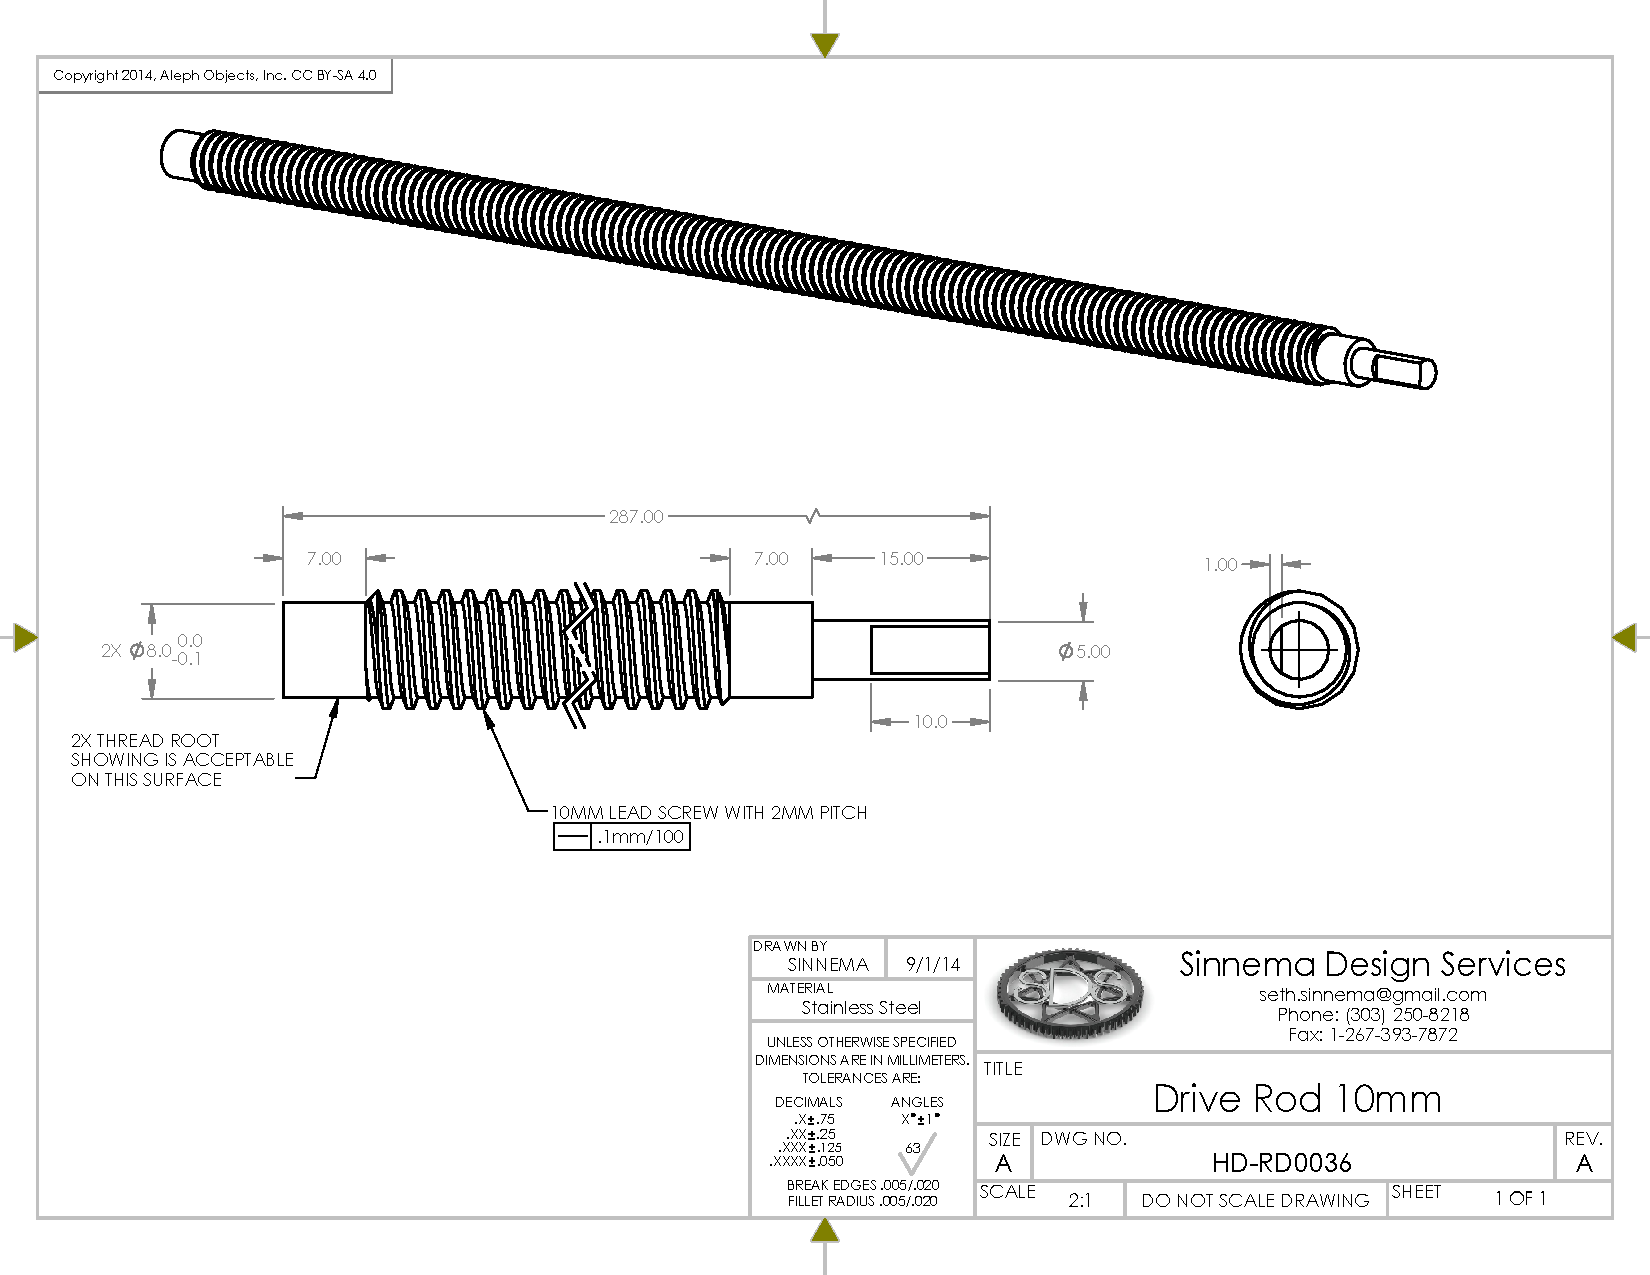
\includepdf[addtolist={1,figure,{Drive Rod 10mm},drvrod},pages=-,landscape=true,reflect=false,turn=false,fitpaper=true,keepaspectratio=true]{driverod10mm.pdf}

\section{3D Printed Parts}
% PNGs were created thusly:
% Open STL in FreeCAD
% View-->Standard View-->Fit All
% Then hit 0 (zero) for axometric view
% Tools-->Save Picture
% XXX DO NOT USE UNDERSCORES (_) IN THE FILENAME!!! XXX

\section{Bed}
\begin{figure}[H]
\centering
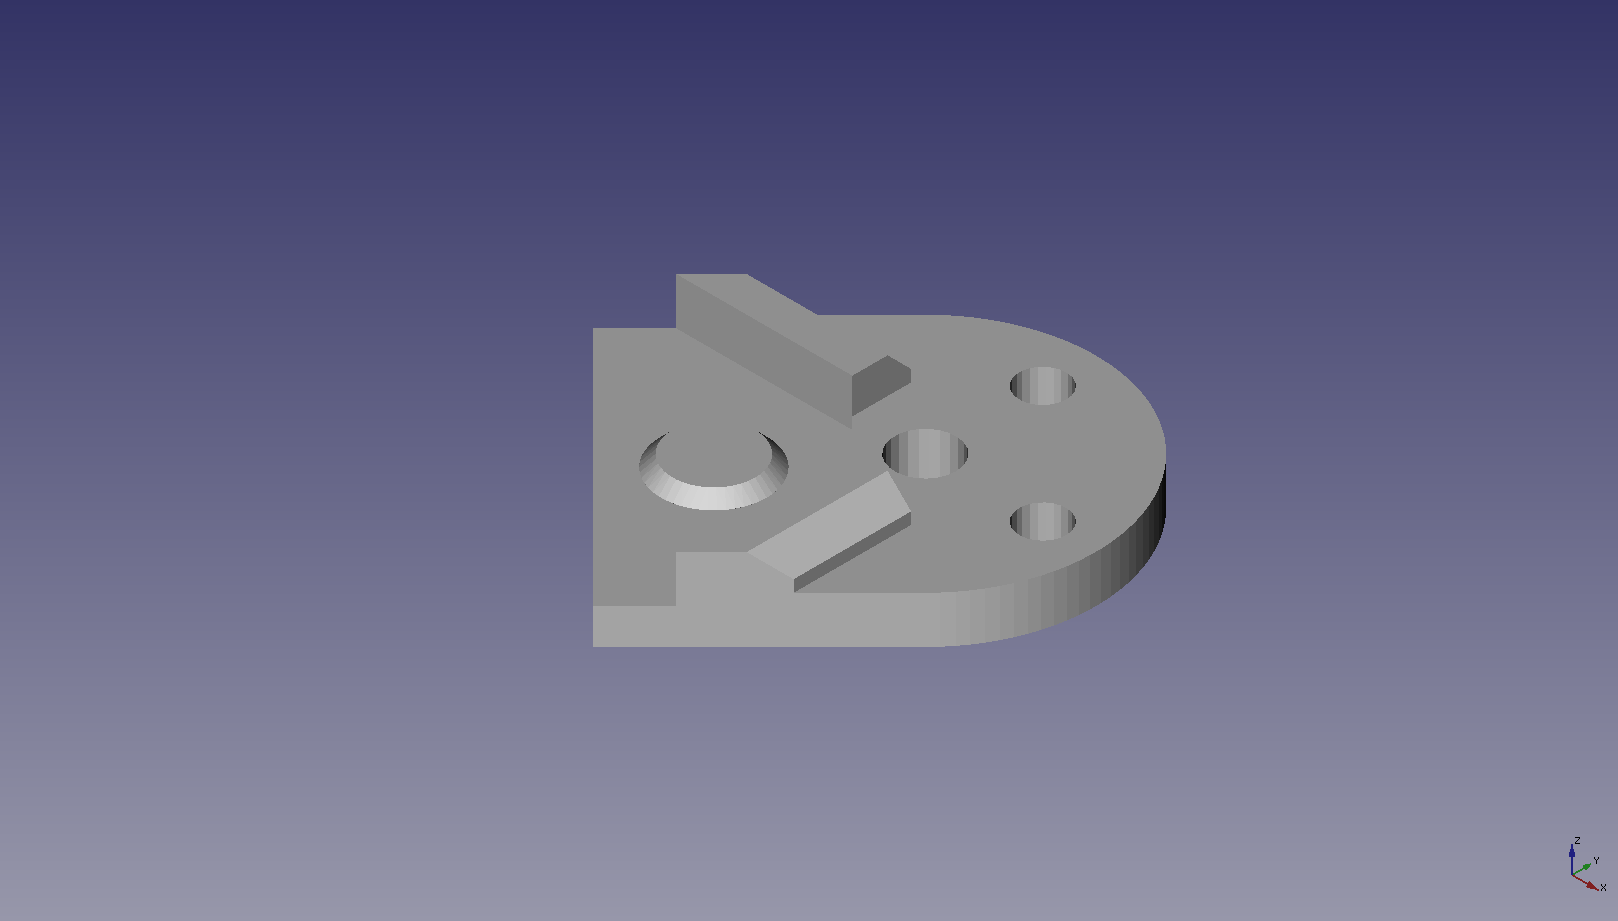
\includegraphics[keepaspectratio=true,angle=0,height=1.0\textheight,width=1.0\textwidth]{STL/bedcorner.stl.png}
\caption{3D Printed Bed Corner Render}
\label{fig:bedcornerrender}
\end{figure}

\section{Extruder}
\begin{figure}[H]
\centering
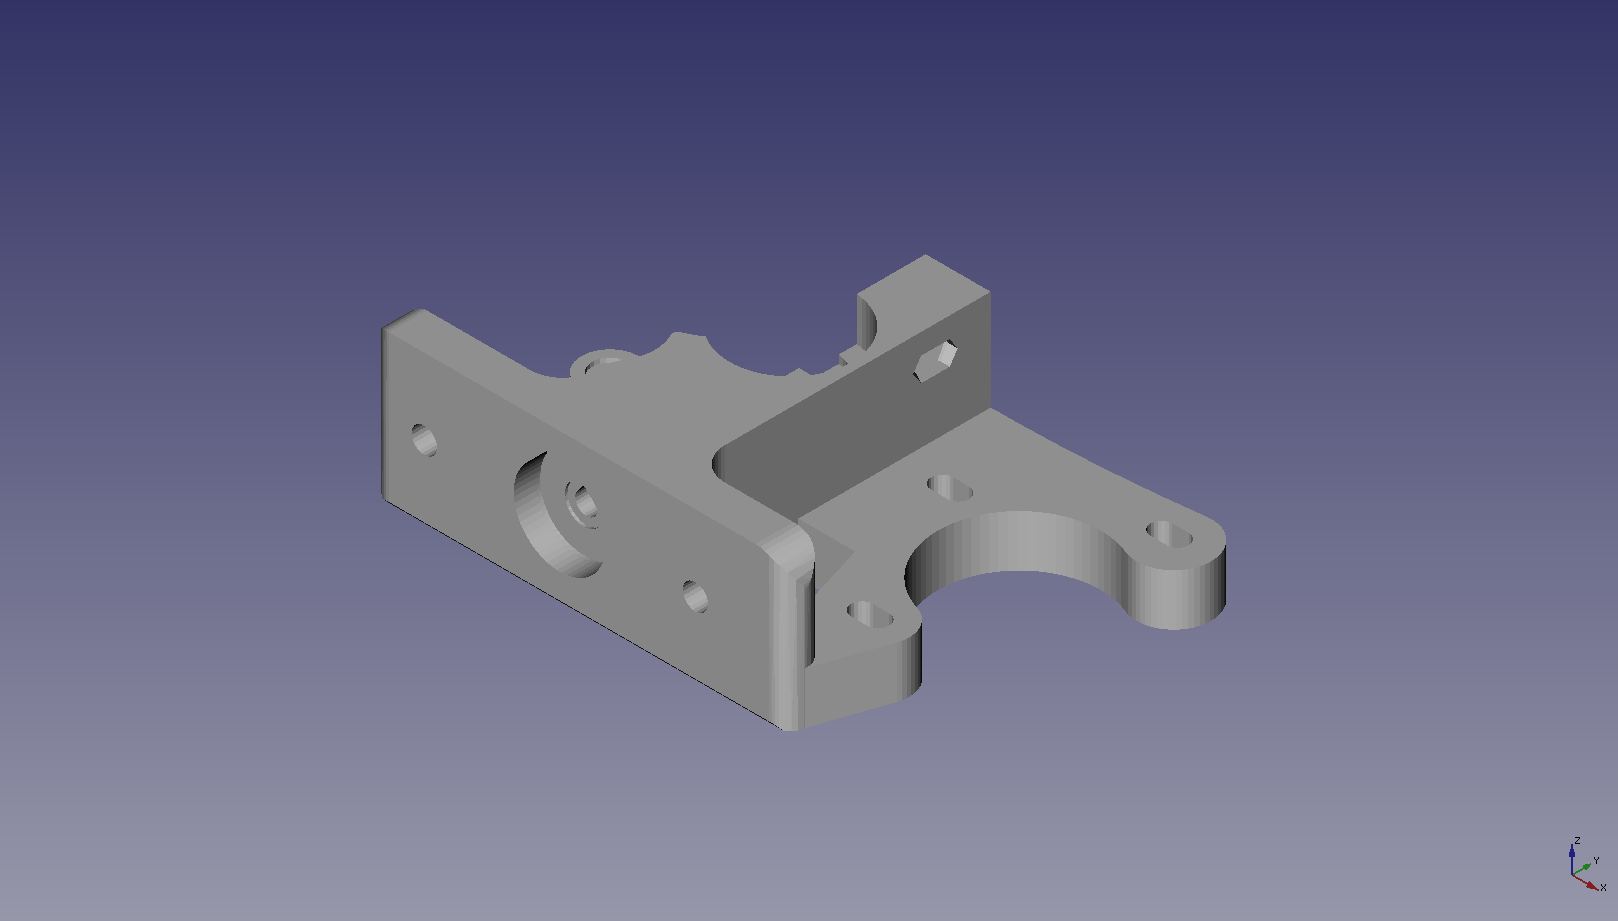
\includegraphics[keepaspectratio=true,angle=0,height=1.0\textheight,width=1.0\textwidth]{STL/extruderbody.stl.png}
\caption{3D Printed Extruder Body Render}
\label{fig:extruderbodyrender}
\end{figure}

\begin{figure}[H]
\centering
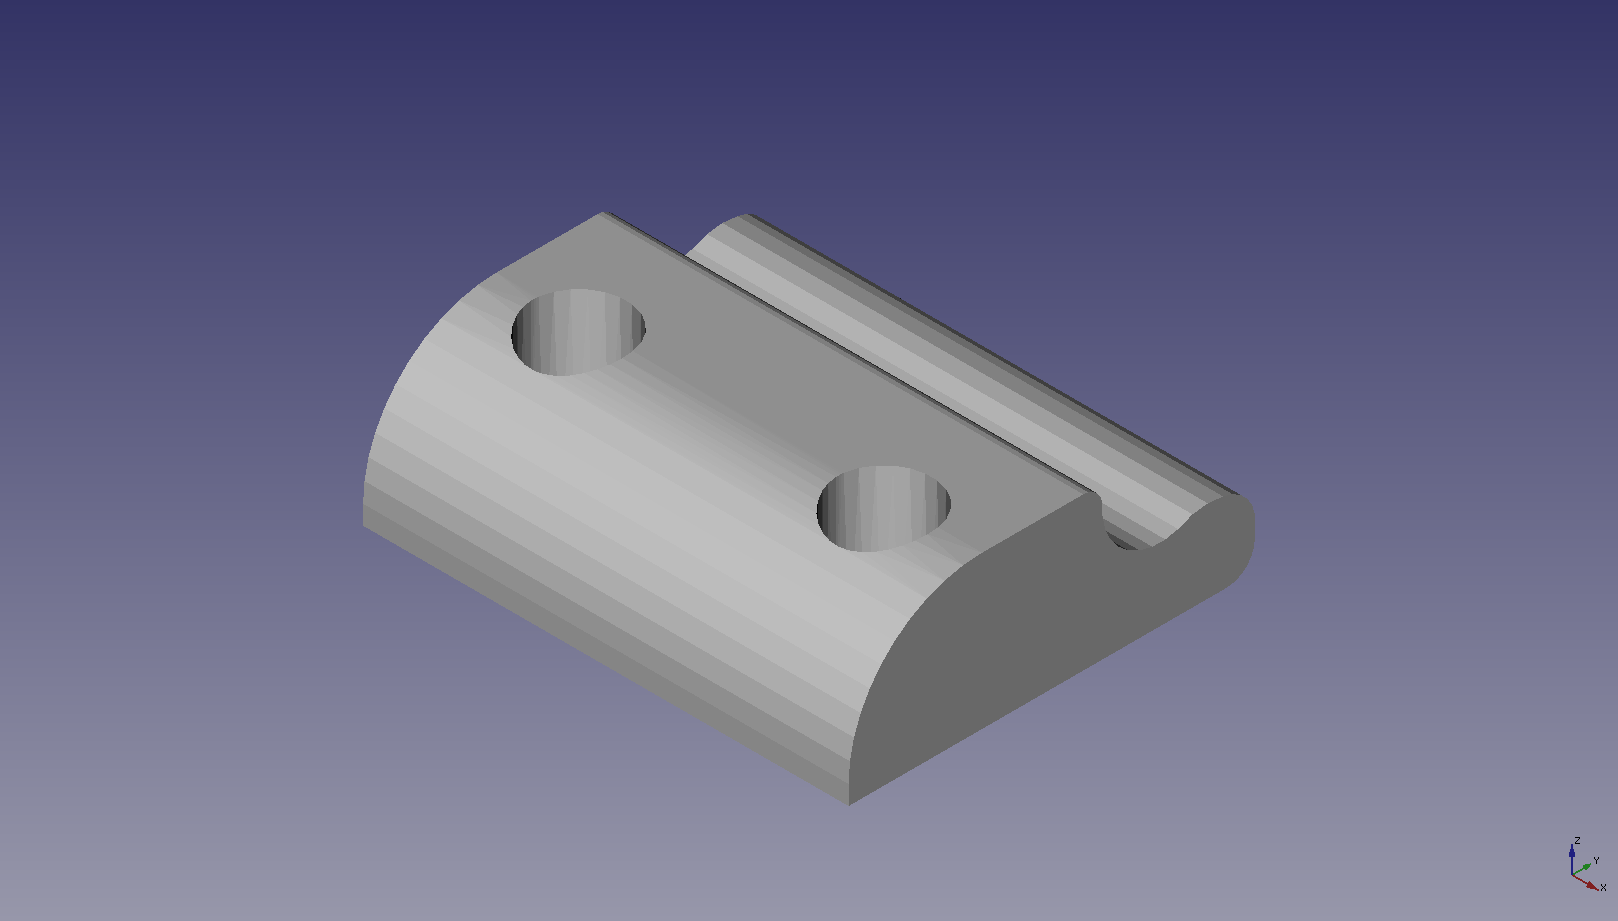
\includegraphics[keepaspectratio=true,angle=0,height=1.0\textheight,width=1.0\textwidth]{STL/extruderlatch.stl.png}
\caption{3D Printed Extruder Latch Render}
\label{fig:extruderlatchrender}
\end{figure}

\begin{figure}[H]
\centering
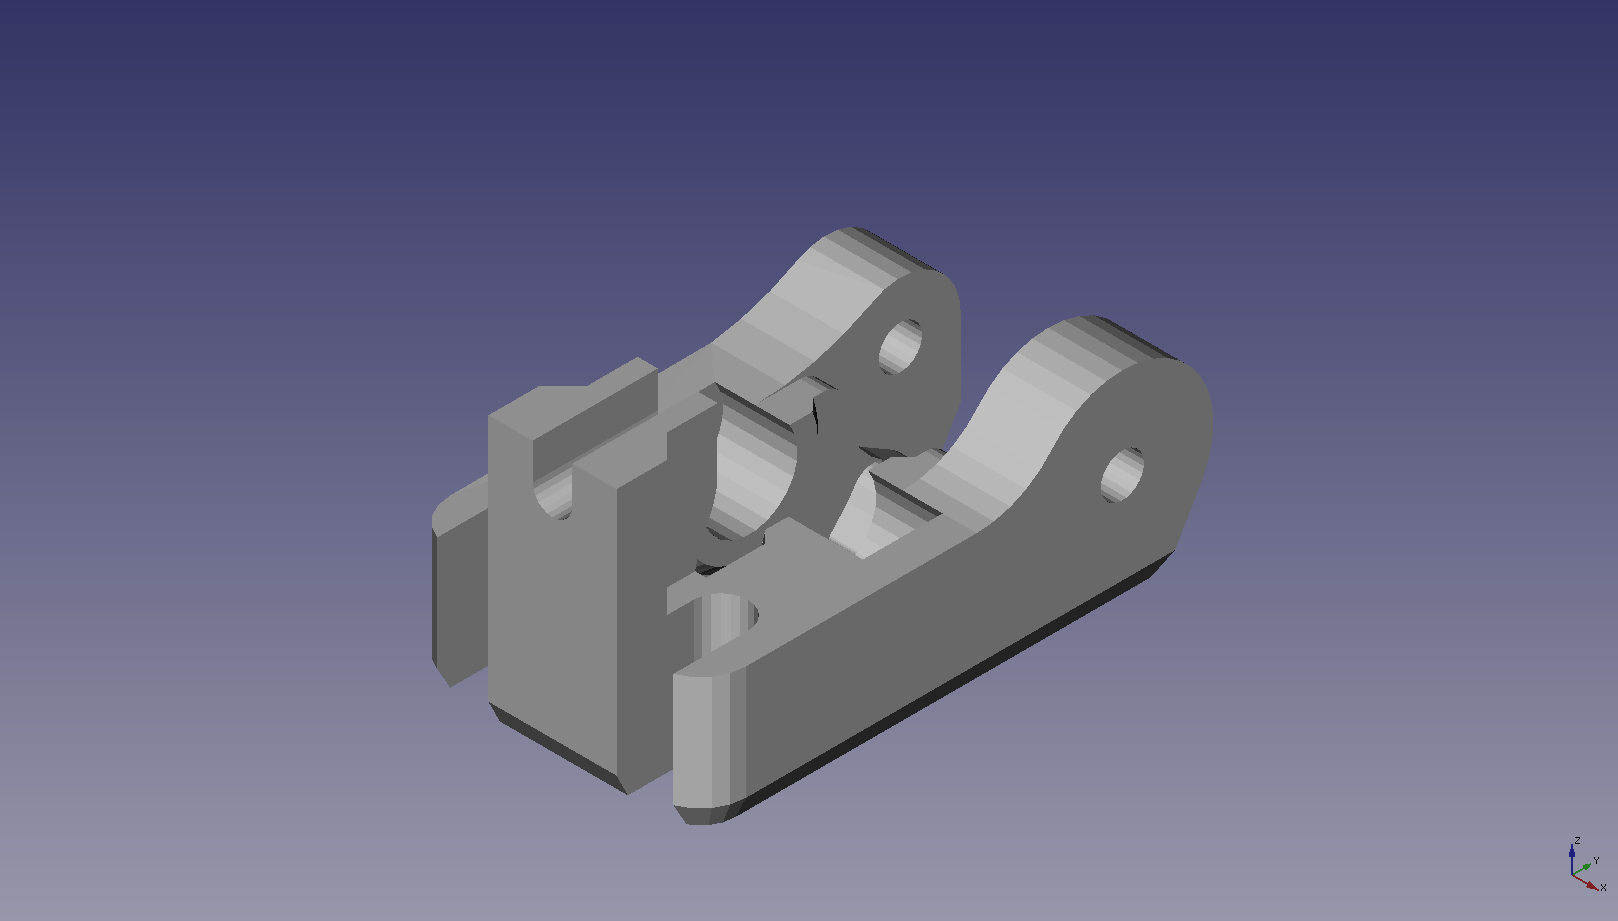
\includegraphics[keepaspectratio=true,angle=0,height=1.0\textheight,width=1.0\textwidth]{STL/idler.stl.png}
\caption{3D Printed Idler Render}
\label{fig:idlerrender}
\end{figure}

\begin{figure}[H]
\centering
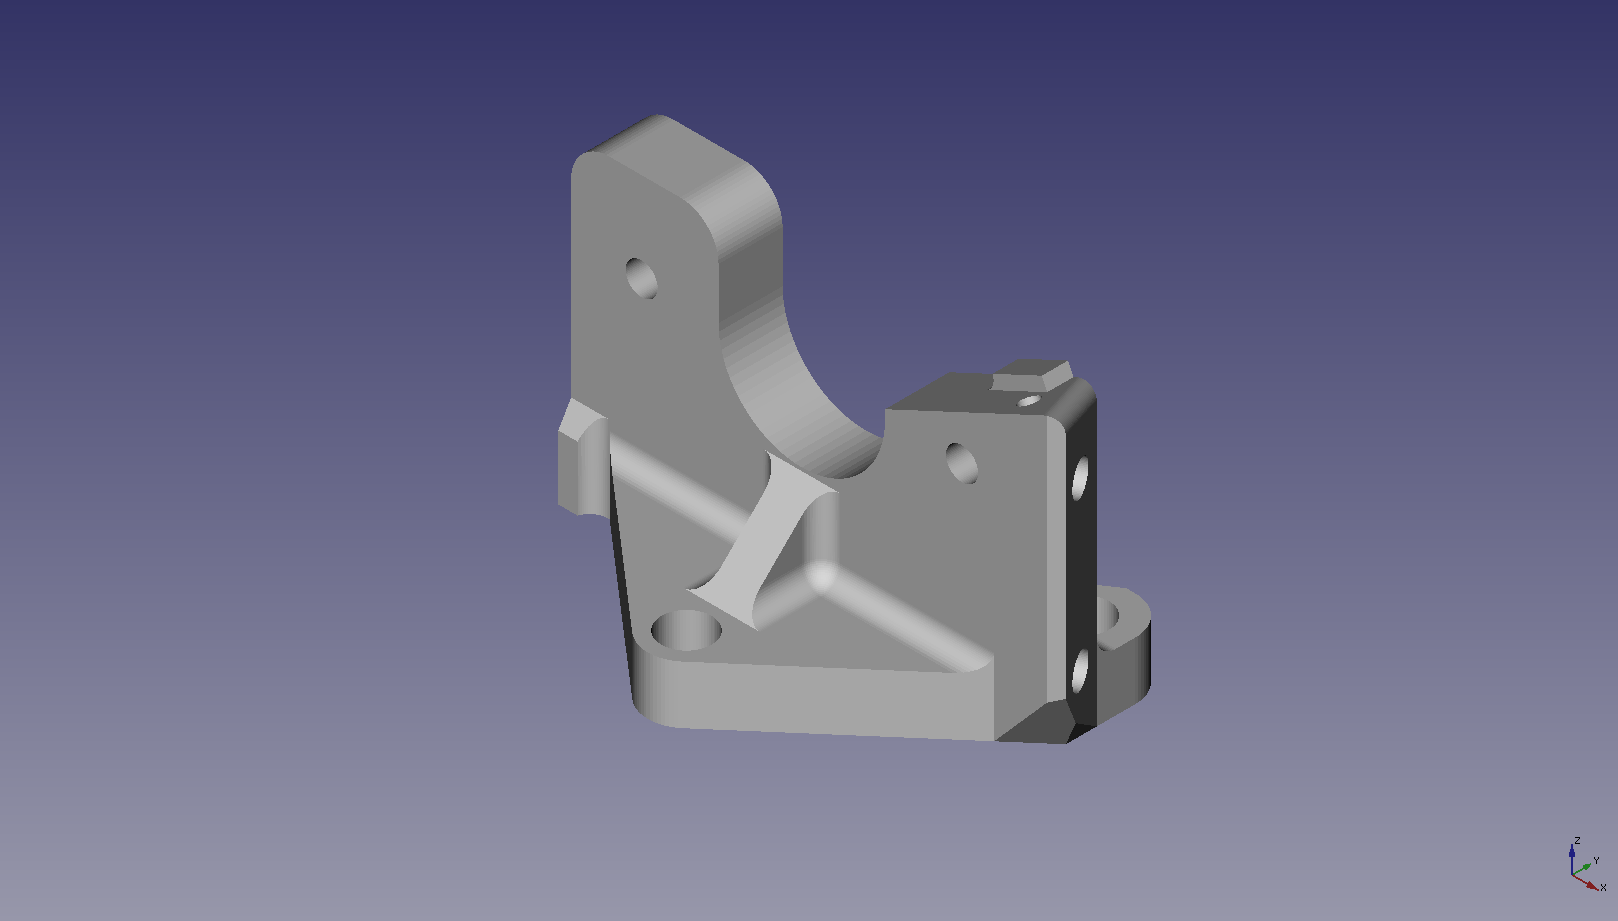
\includegraphics[keepaspectratio=true,angle=0,height=1.0\textheight,width=1.0\textwidth]{STL/extrudermount.stl.png}
\caption{3D Printed Extruder Mount Render}
\label{fig:extrudermountrender}
\end{figure}

\begin{figure}[H]
\centering
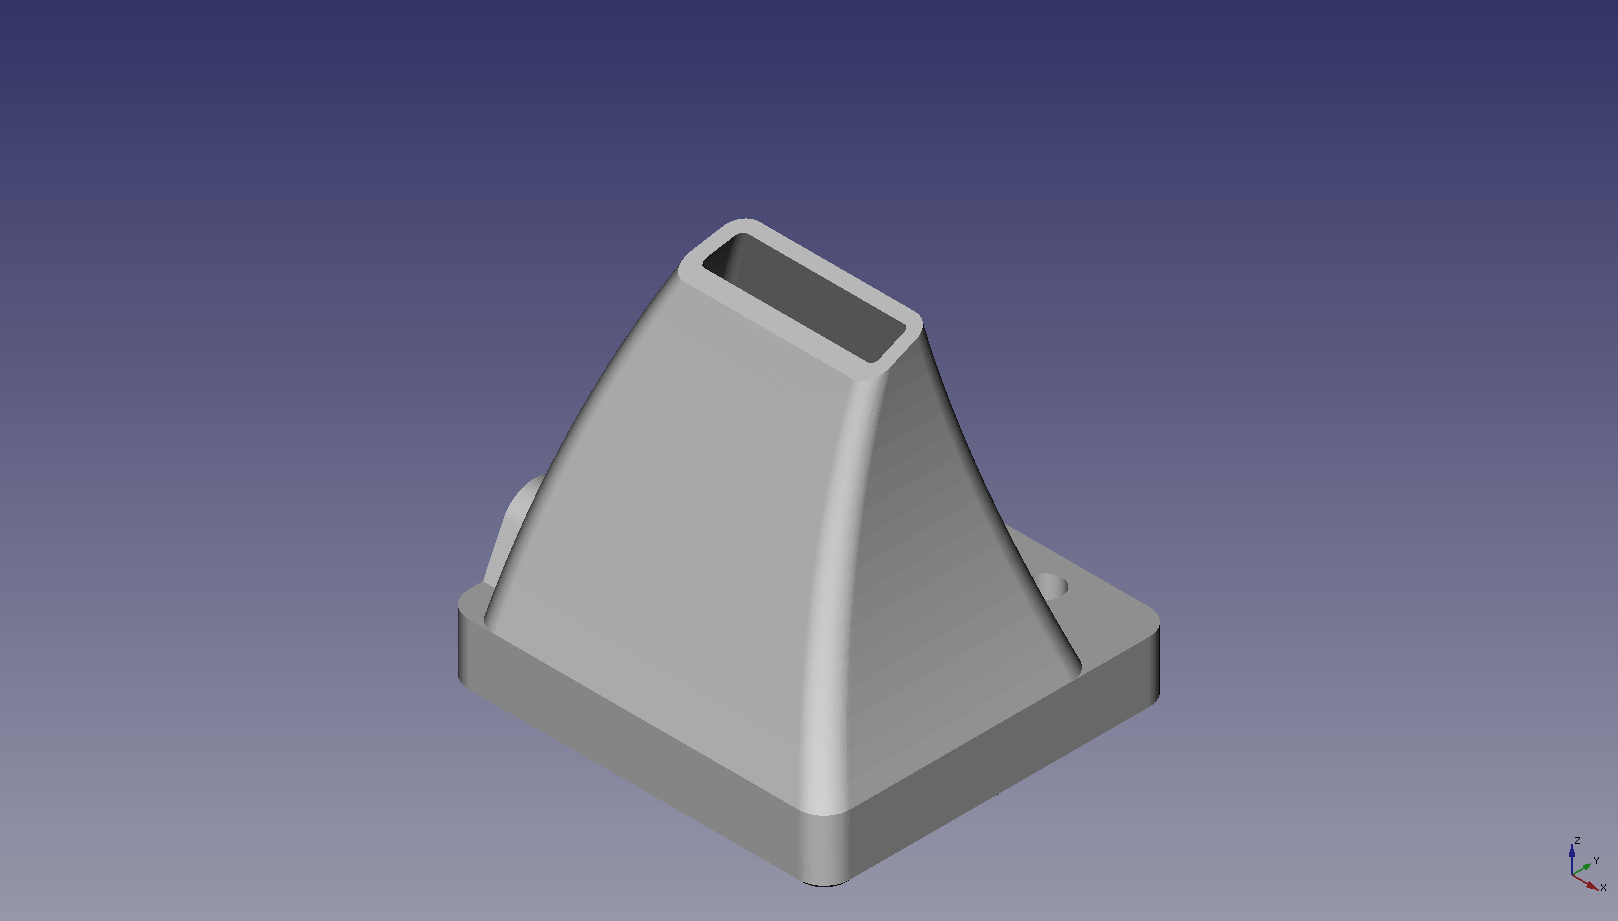
\includegraphics[keepaspectratio=true,angle=0,height=1.0\textheight,width=1.0\textwidth]{STL/fanmount.stl.png}
\caption{3D Printed Fan Mount Render}
\label{fig:fanmountrender}
\end{figure}

\begin{figure}[H]
\centering
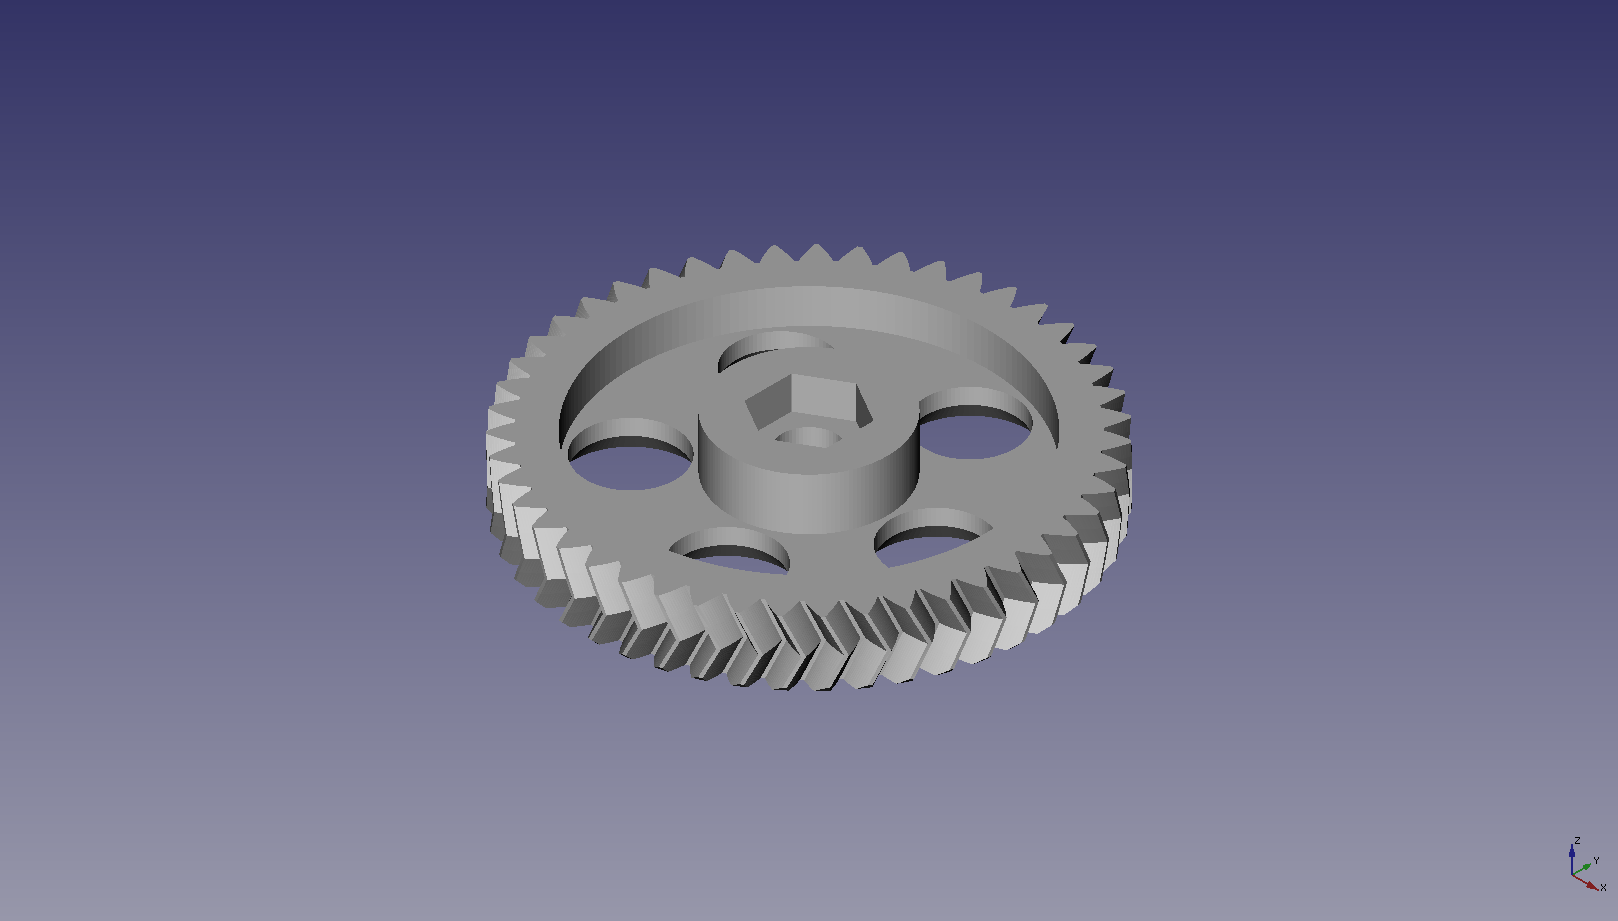
\includegraphics[keepaspectratio=true,angle=0,height=1.0\textheight,width=1.0\textwidth]{STL/gearlarge.stl.png}
\caption{3D Printed Large Gear Render}
\label{fig:gearlargerender}
\end{figure}

\begin{figure}[H]
\centering
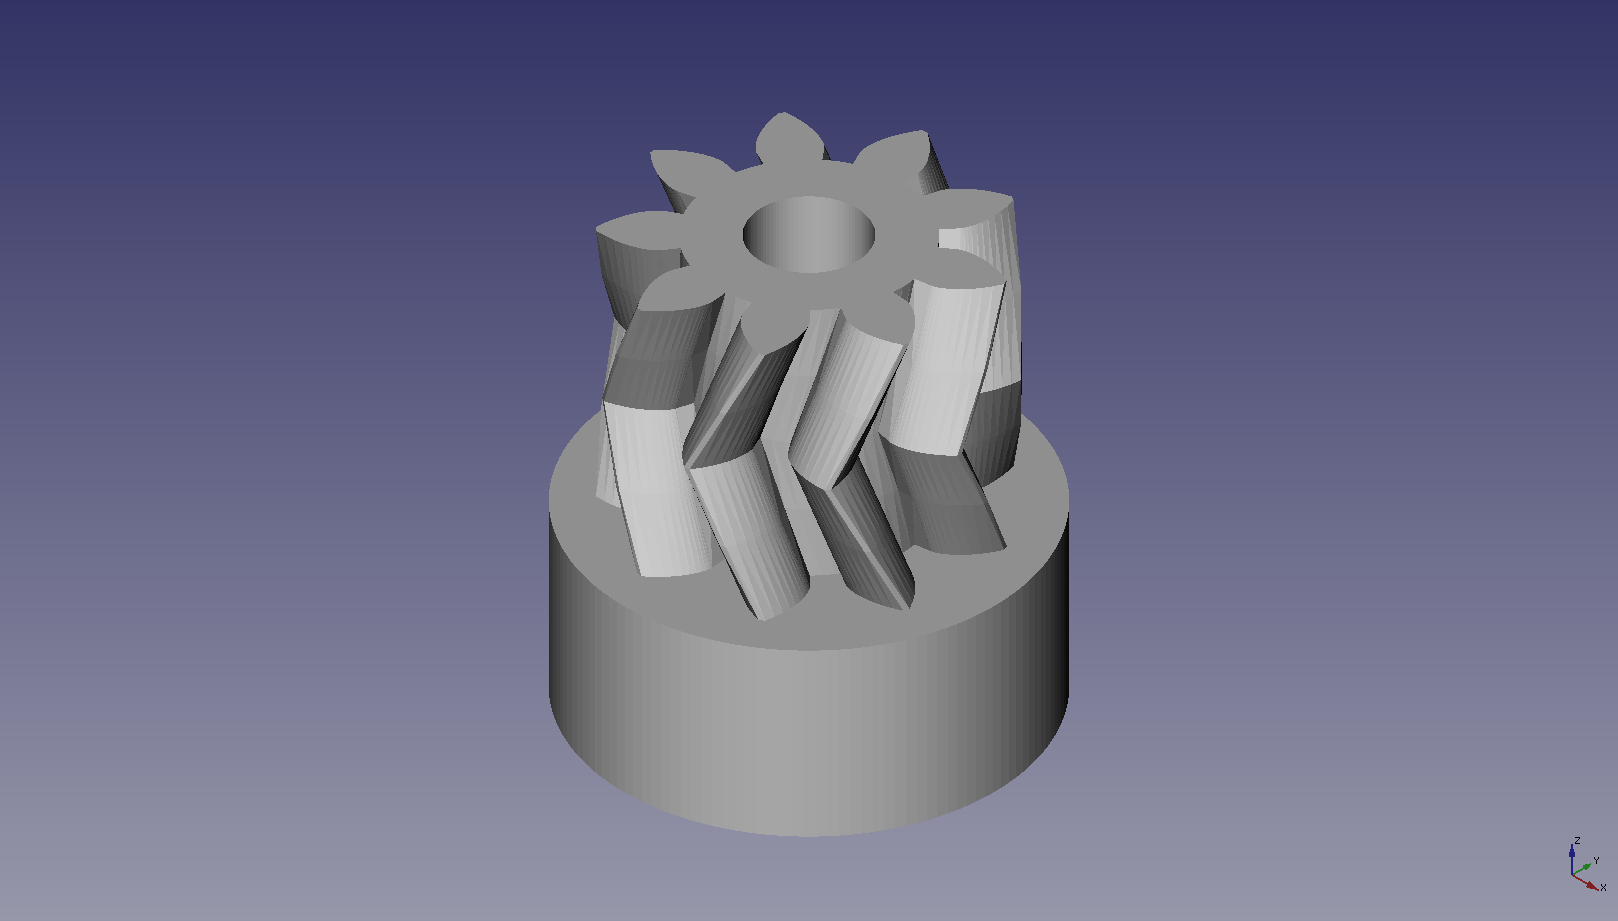
\includegraphics[keepaspectratio=true,angle=0,height=1.0\textheight,width=1.0\textwidth]{STL/gearsmall.stl.png}
\caption{3D Printed Small Gear Render}
\label{fig:gearsmallrender}
\end{figure}

\section{Spool}

\begin{figure}[H]
\centering
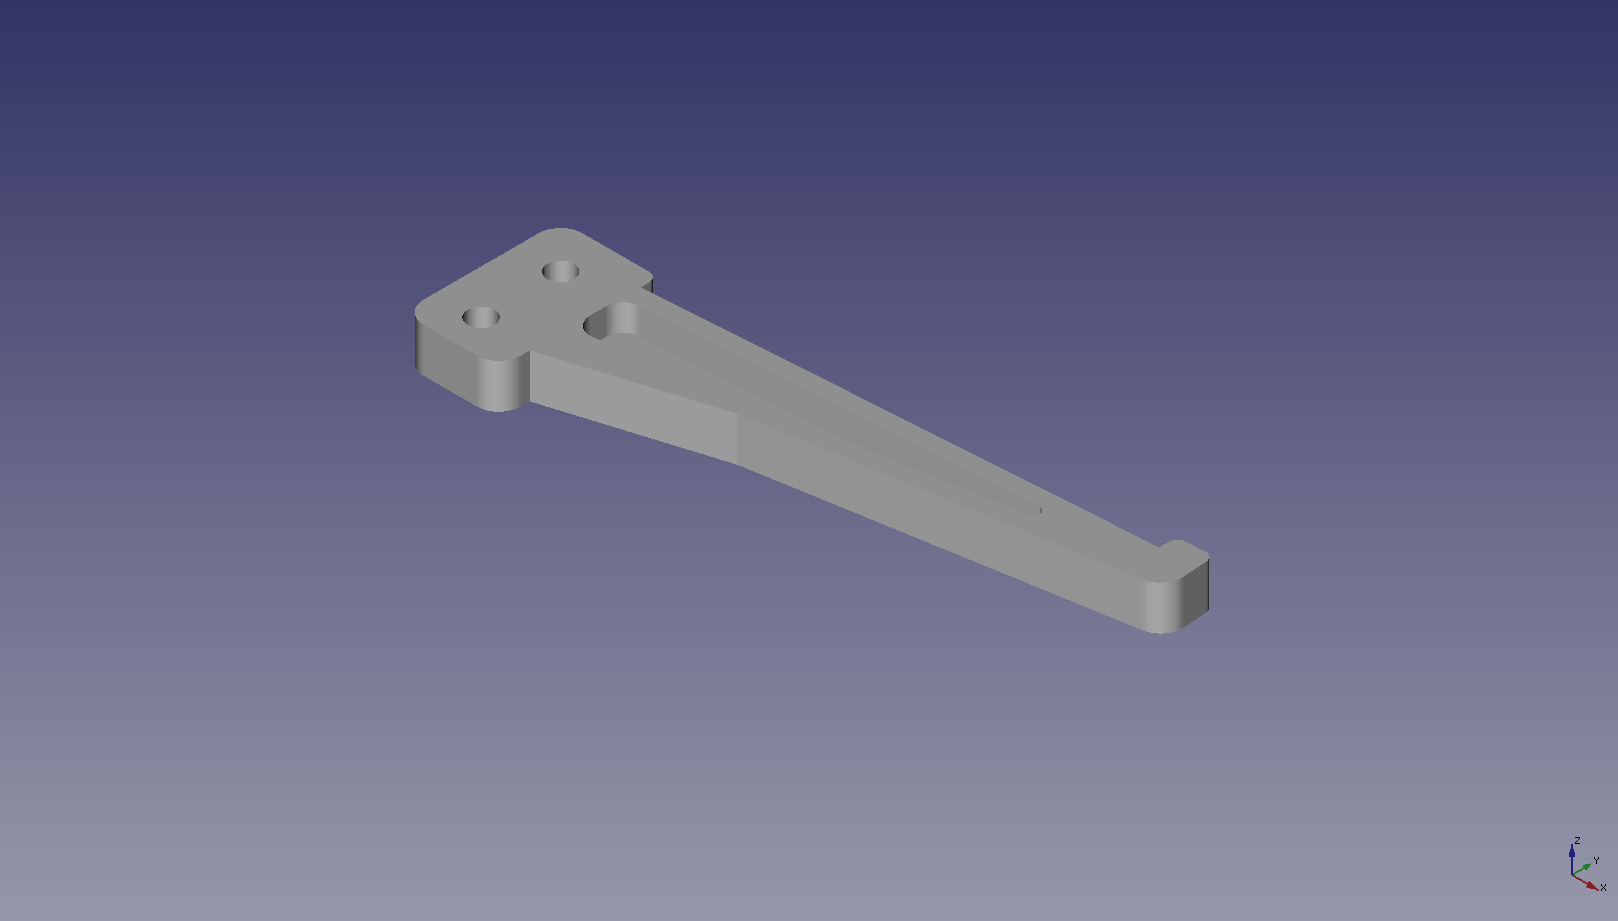
\includegraphics[keepaspectratio=true,angle=0,height=1.0\textheight,width=1.0\textwidth]{STL/spoolarm.stl.png}
\caption{3D Printed Spool Arm Render}
\label{fig:spoolarmrender}
\end{figure}

\begin{figure}[H]
\centering
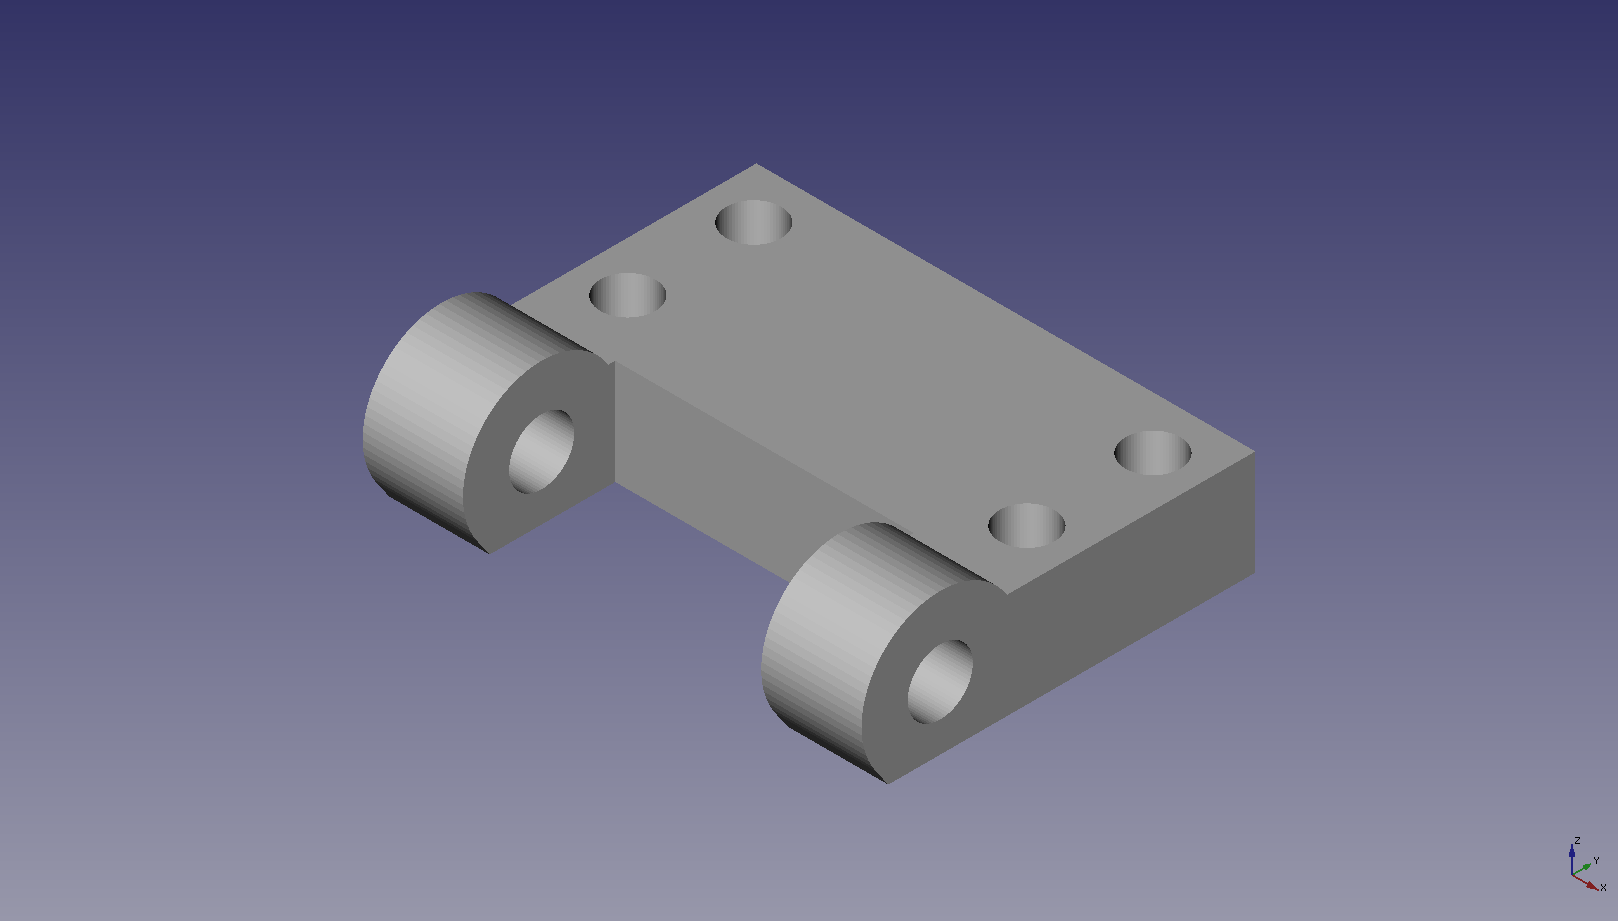
\includegraphics[keepaspectratio=true,angle=0,height=1.0\textheight,width=1.0\textwidth]{STL/spoolhinge.stl.png}
\caption{3D Printed Spool Hinge Render}
\label{fig:spoolhingerender}
\end{figure}

\begin{figure}[H]
\centering
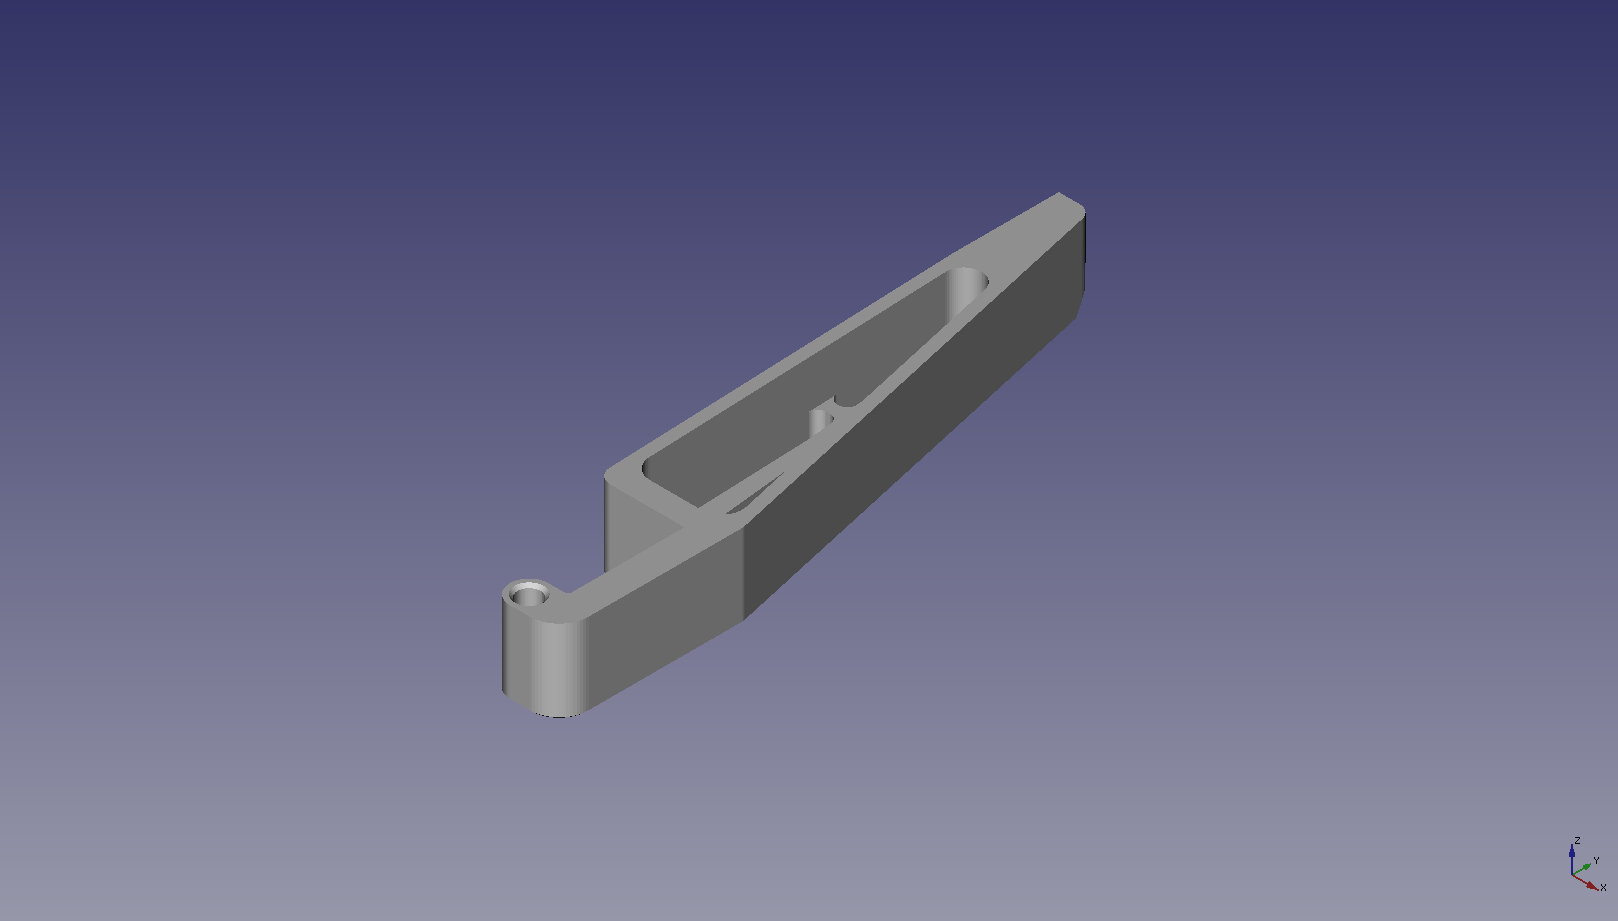
\includegraphics[keepaspectratio=true,angle=0,height=1.0\textheight,width=1.0\textwidth]{STL/spoolmount.stl.png}
\caption{3D Printed Spool Mount Render}
\label{fig:spoolmountrender}
\end{figure}

\section{X}

\begin{figure}[H]
\centering
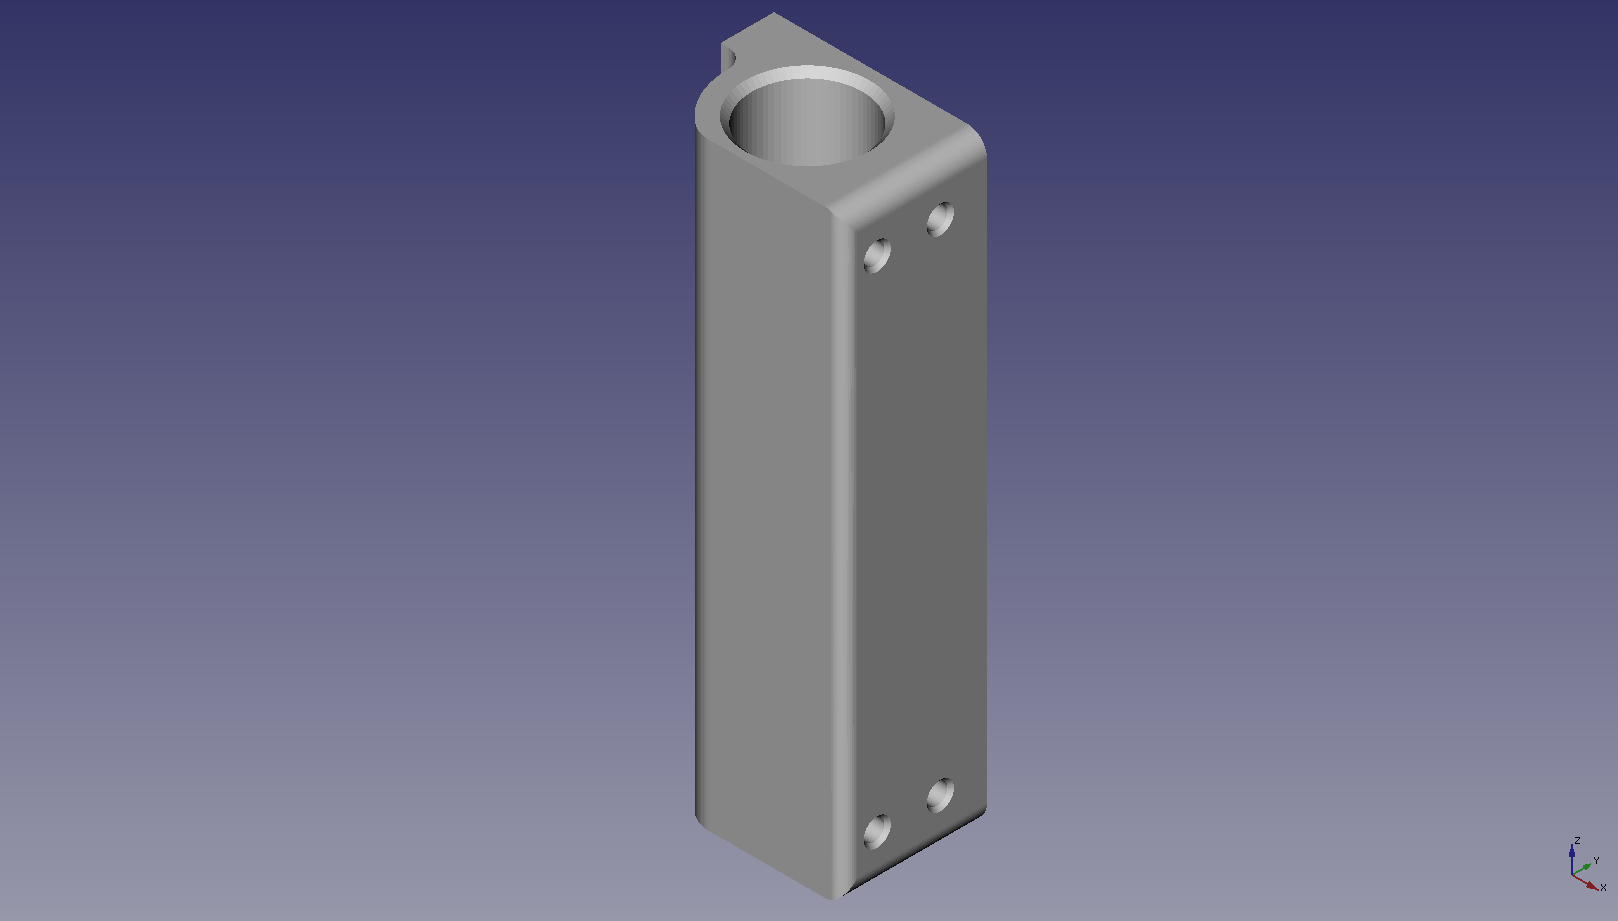
\includegraphics[keepaspectratio=true,angle=0,height=1.0\textheight,width=1.0\textwidth]{STL/doublebearingholder.stl.png}
\caption{3D Printed Double Bearing Holder Render}
\label{fig:doublebearingholderrender}
\end{figure}

\begin{figure}[H]
\centering
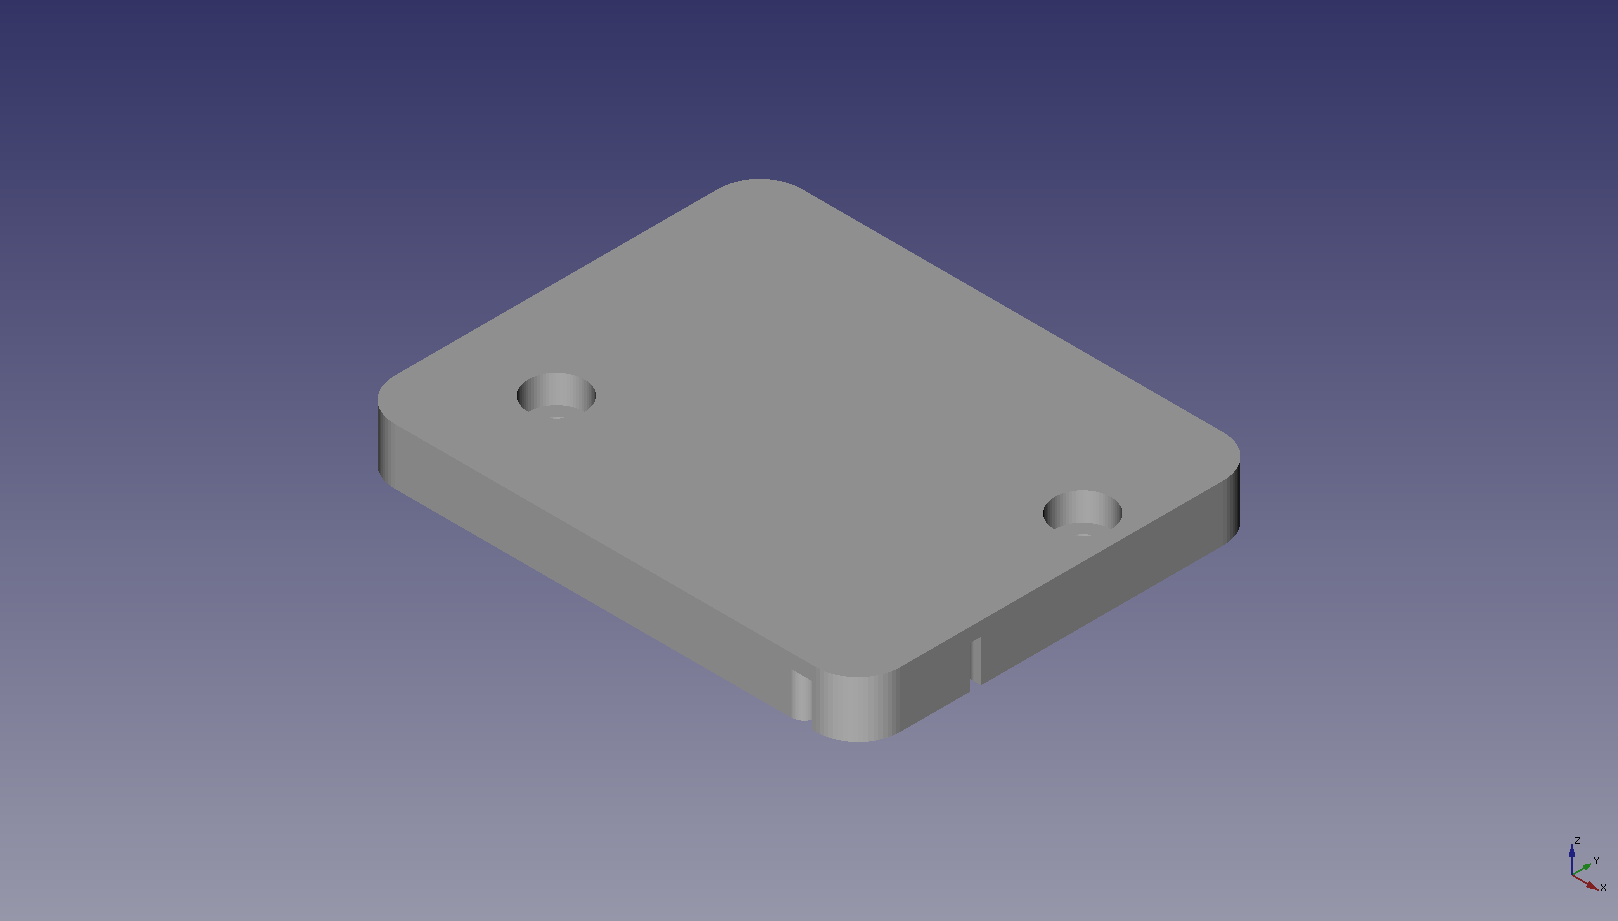
\includegraphics[keepaspectratio=true,angle=0,height=1.0\textheight,width=1.0\textwidth]{STL/xcarriagecover.stl.png}
\caption{3D Printed X Carriage Cover Render}
\label{fig:xcarriagecoverrender}
\end{figure}

\begin{figure}[H]
\centering
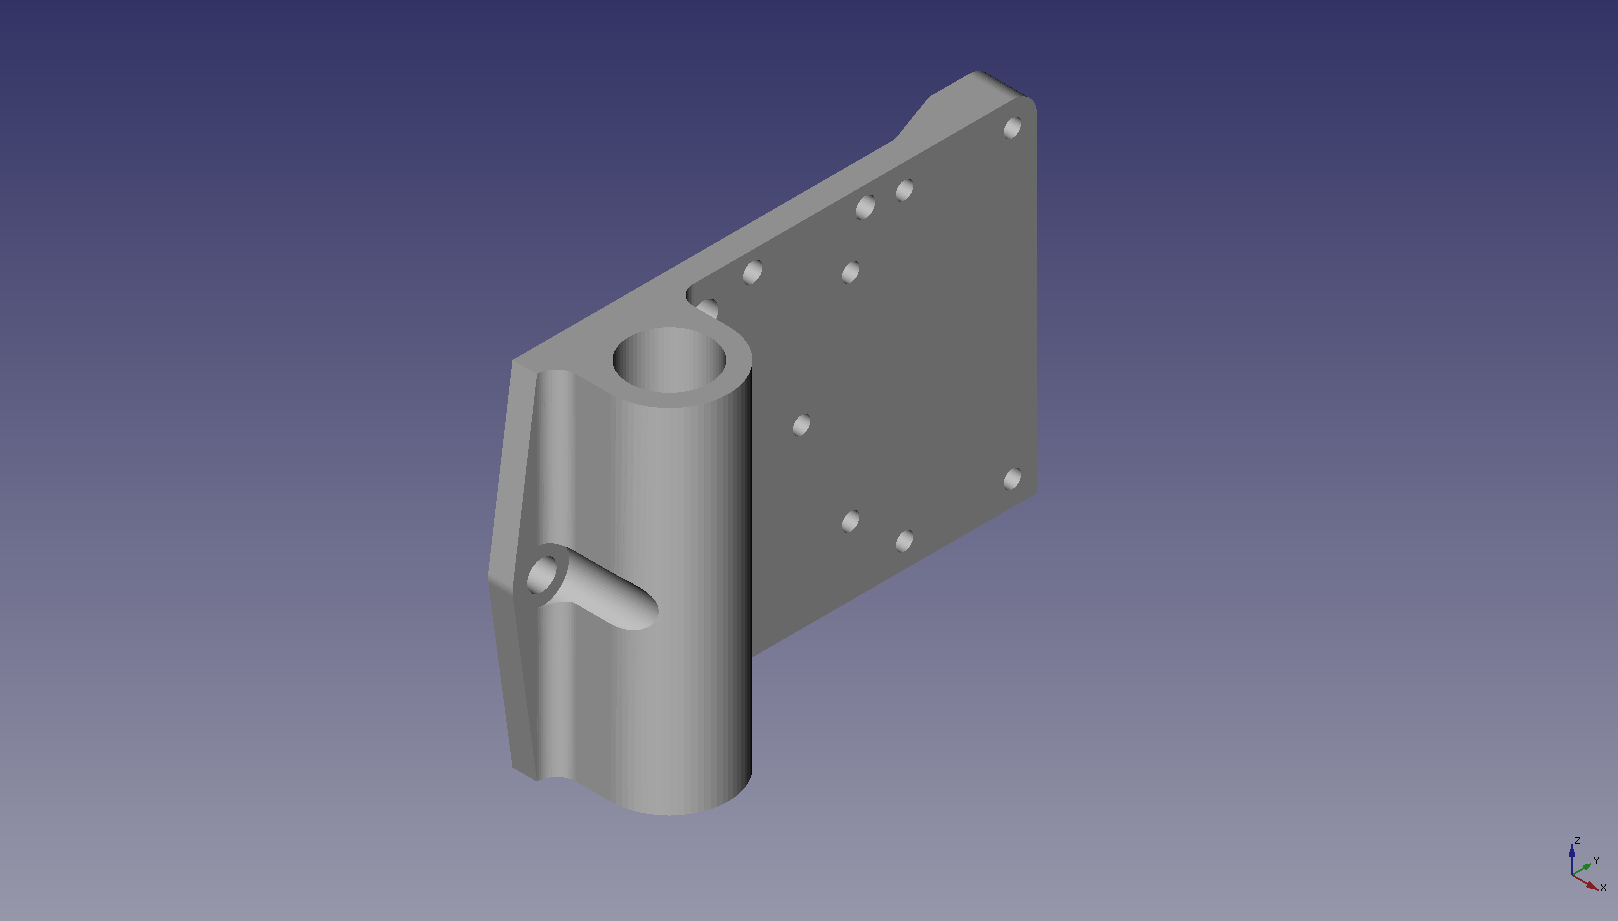
\includegraphics[keepaspectratio=true,angle=0,height=1.0\textheight,width=1.0\textwidth]{STL/xcarriage.stl.png}
\caption{3D Printed X Carriage Render}
\label{fig:xcarriagerender}
\end{figure}

\begin{figure}[H]
\centering
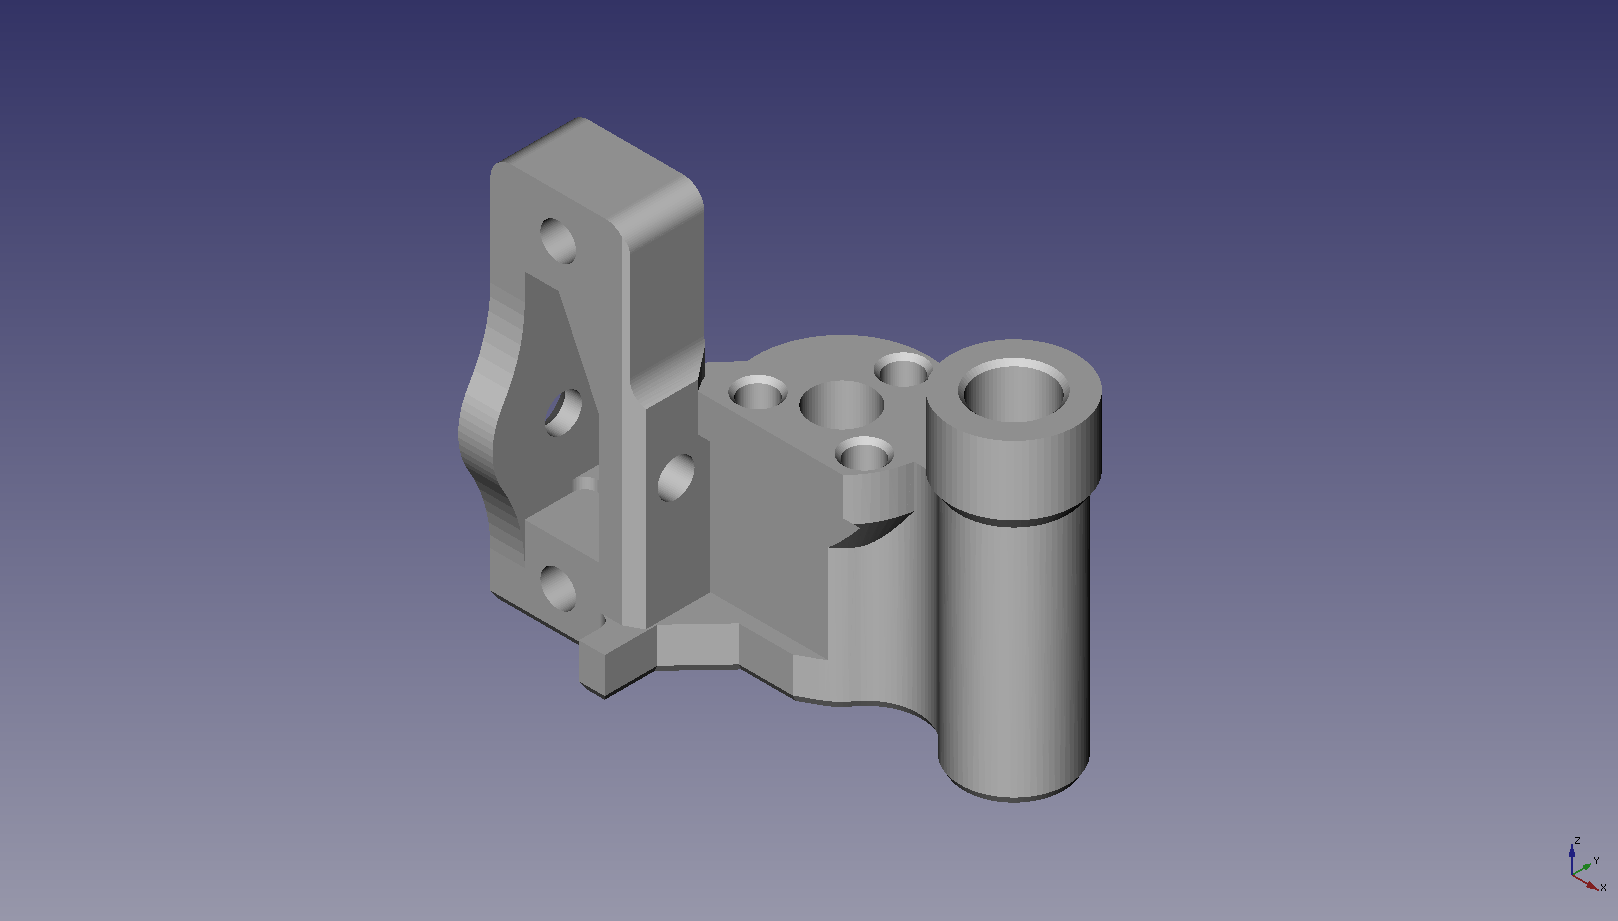
\includegraphics[keepaspectratio=true,angle=0,height=1.0\textheight,width=1.0\textwidth]{STL/xendidler.stl.png}
\caption{3D Printed X End Idler Render}
\label{fig:xendidlerrender}
\end{figure}

\begin{figure}[H]
\centering
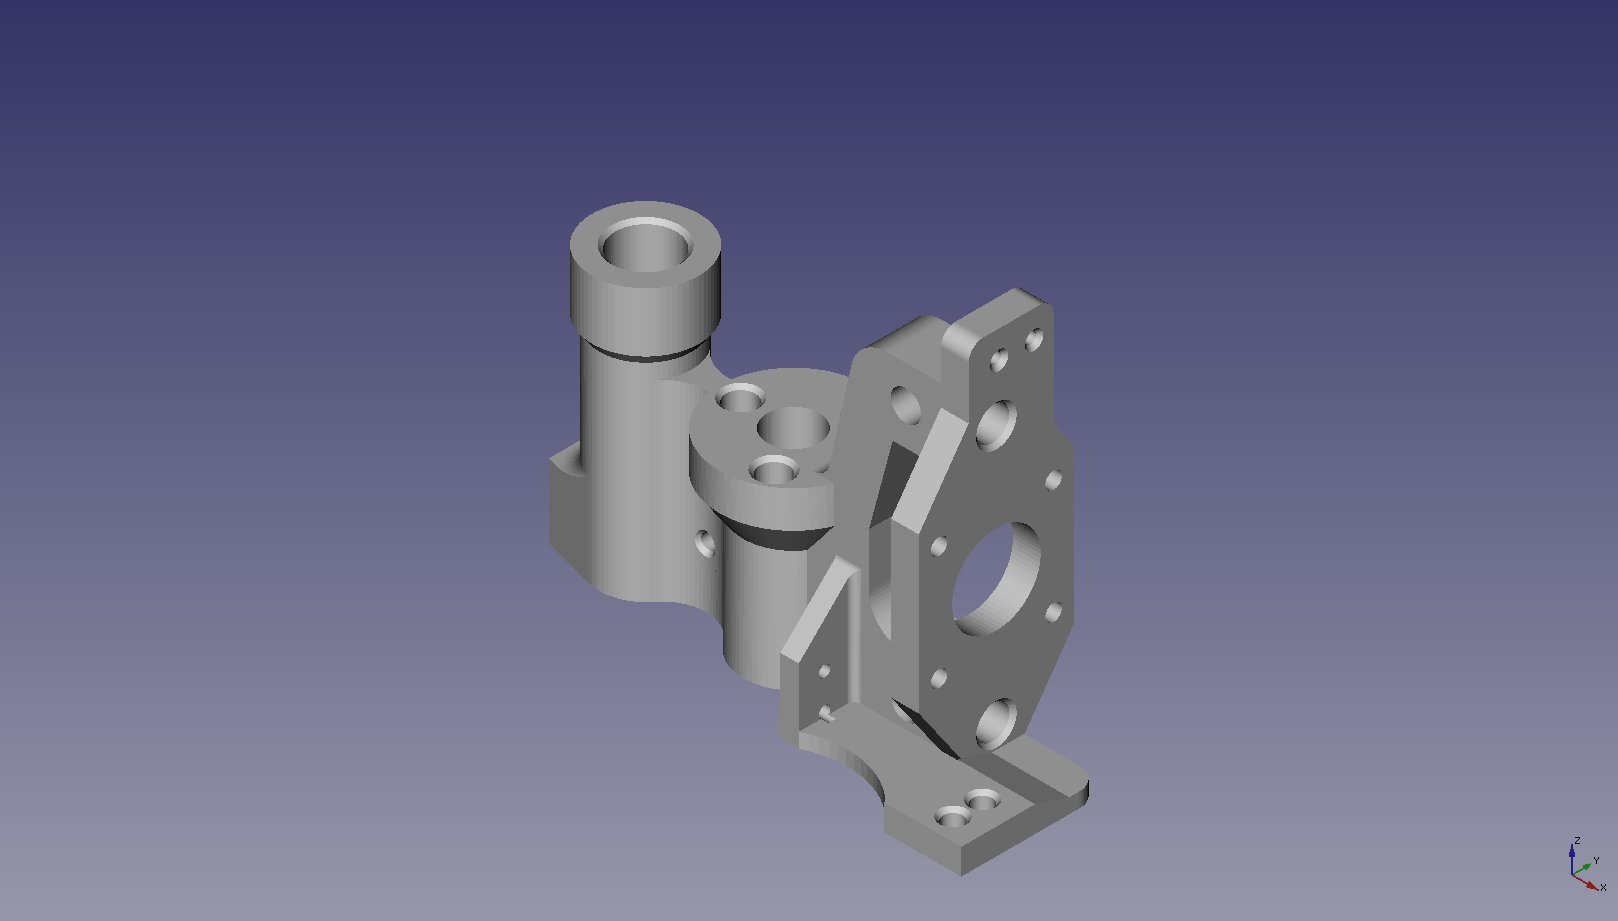
\includegraphics[keepaspectratio=true,angle=0,height=1.0\textheight,width=1.0\textwidth]{STL/xendmotor.stl.png}
\caption{3D Printed X End Motor Render}
\label{fig:render}
\end{figure}

\section{Y}

\begin{figure}[H]
\centering
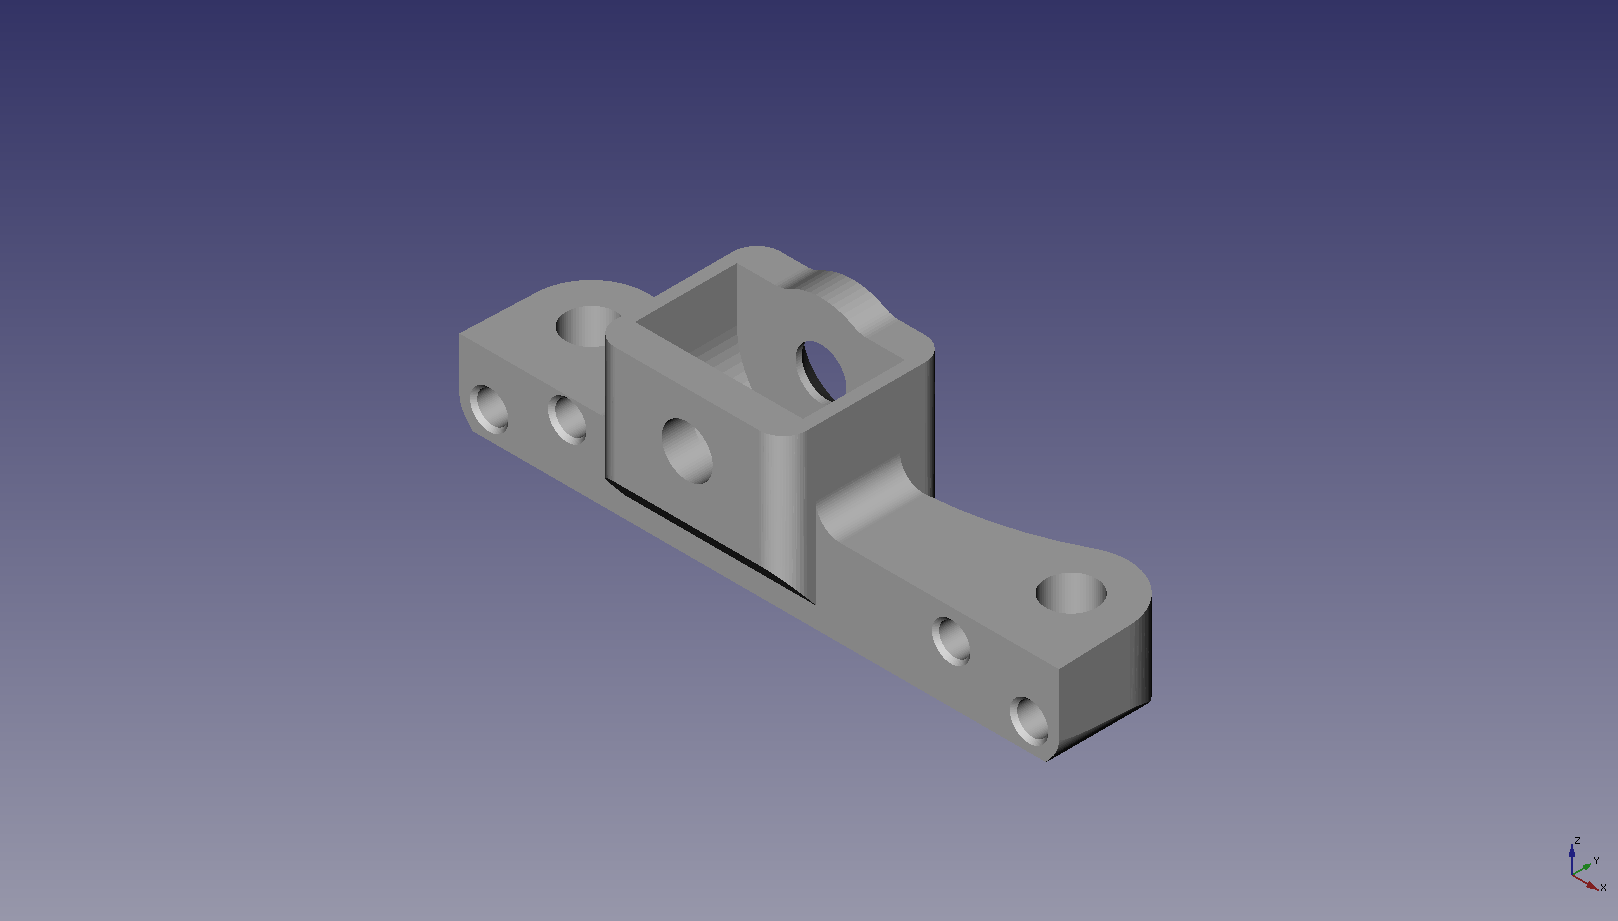
\includegraphics[keepaspectratio=true,angle=0,height=1.0\textheight,width=1.0\textwidth]{STL/yendidler.stl.png}
\caption{3D Printed Y End Idler Render}
\label{fig:render}
\end{figure}

\begin{figure}[H]
\centering
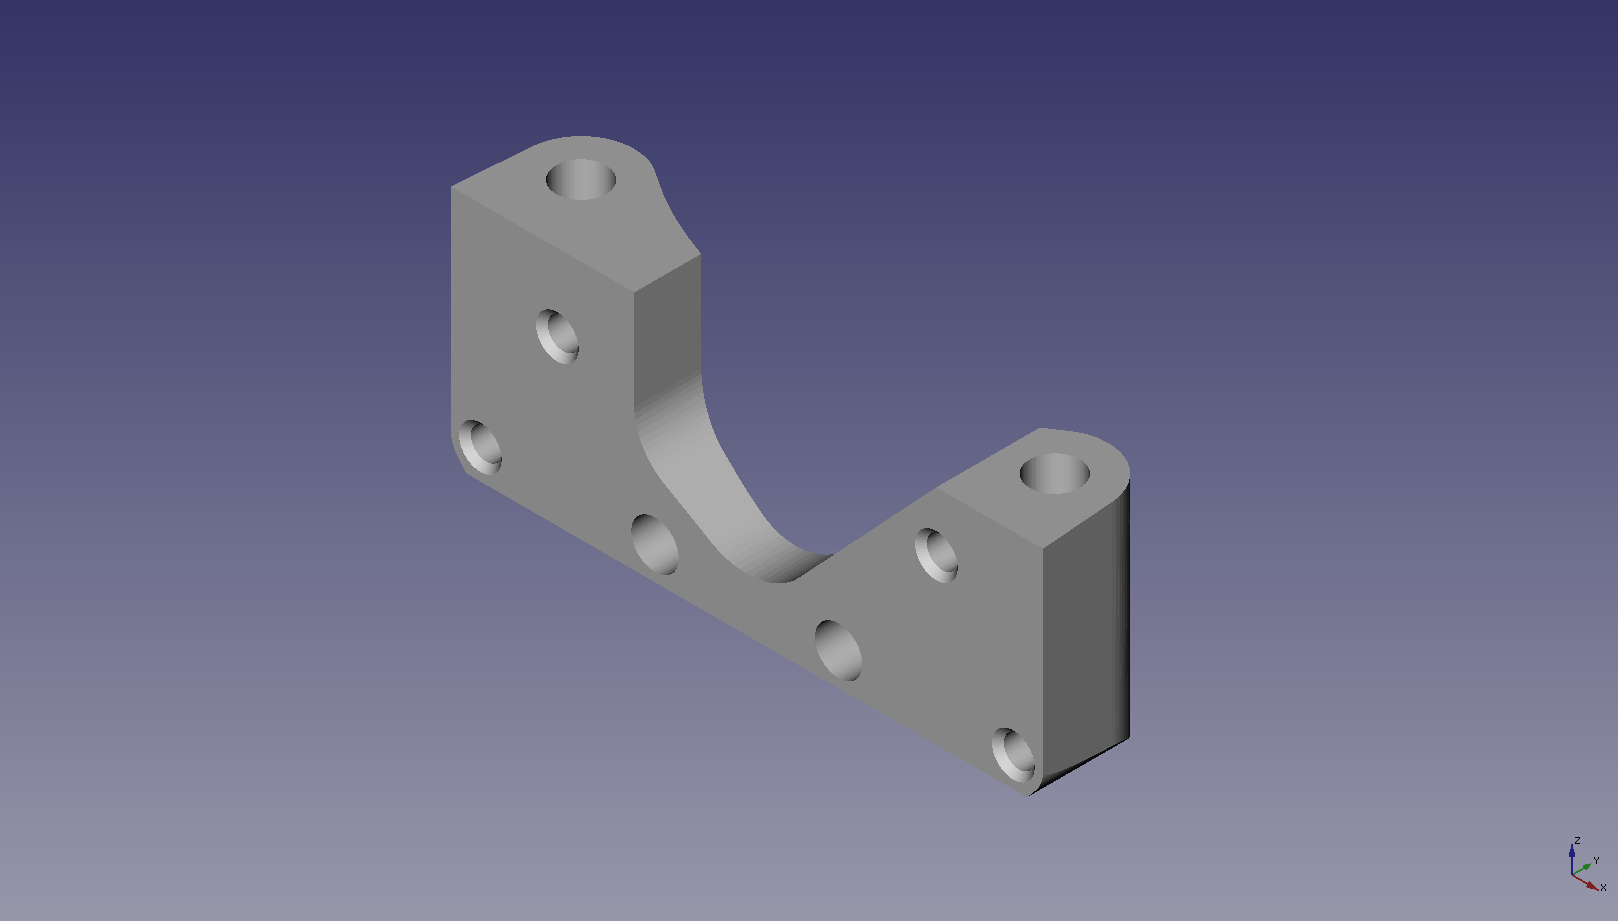
\includegraphics[keepaspectratio=true,angle=0,height=1.0\textheight,width=1.0\textwidth]{STL/yendrodmount.stl.png}
\caption{3D Printed Y End Rod Mount Render}
\label{fig:yendrodmountrender}
\end{figure}

\section{Z}

\begin{figure}[H]
\centering
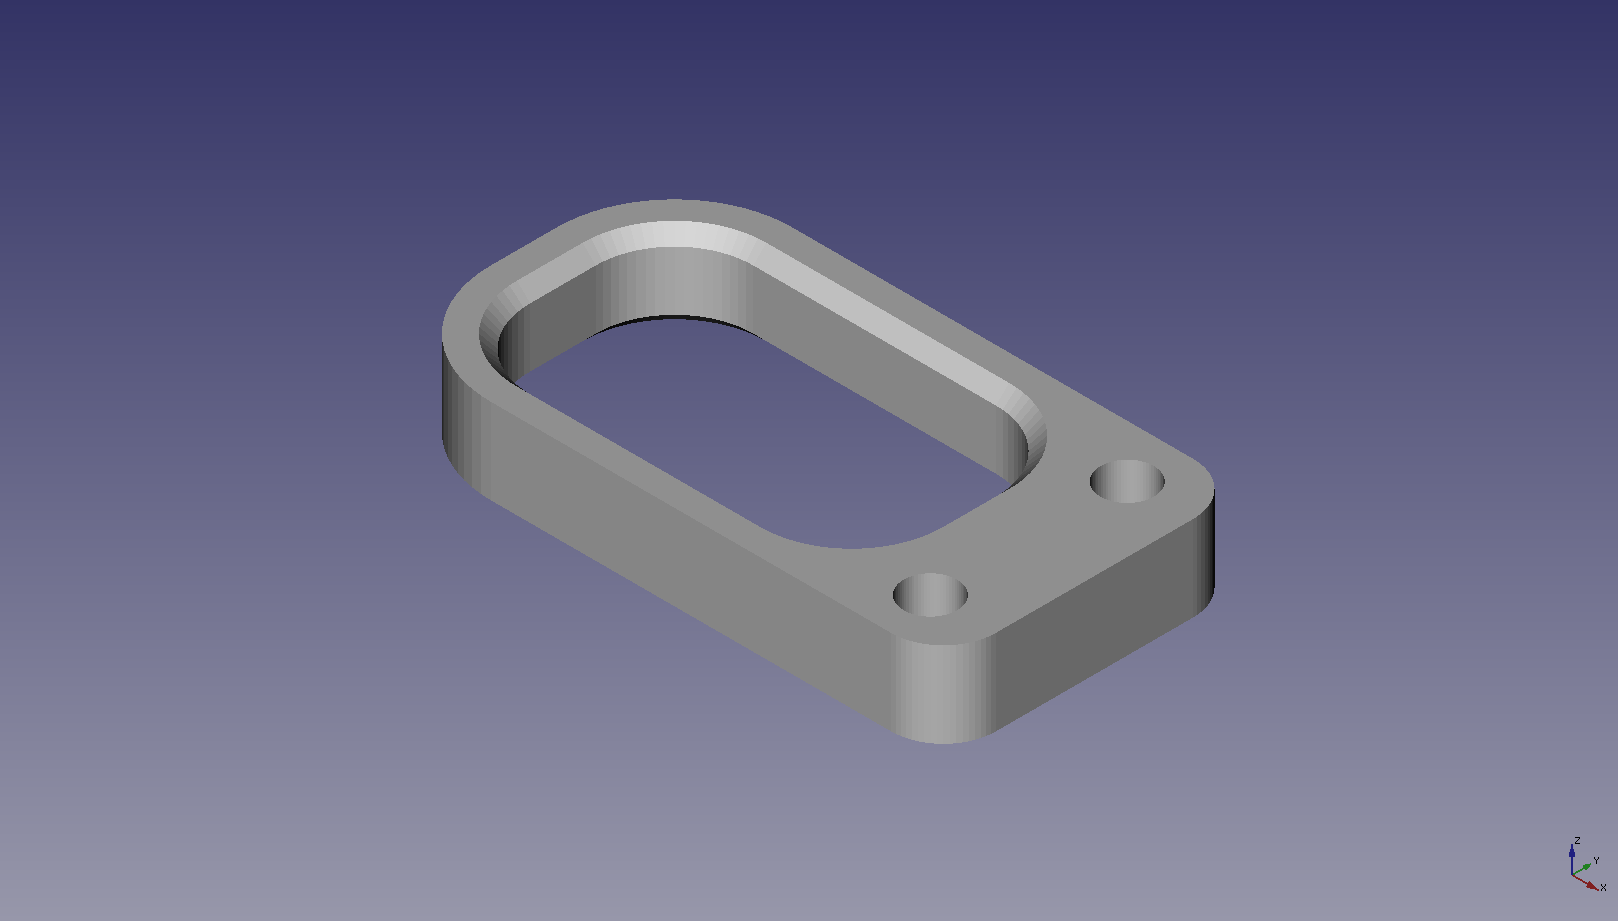
\includegraphics[keepaspectratio=true,angle=0,height=1.0\textheight,width=1.0\textwidth]{STL/lowrelief.stl.png}
\caption{3D Printed Lower Relief Render}
\label{fig:lowreliefrender}
\end{figure}

\begin{figure}[H]
\centering
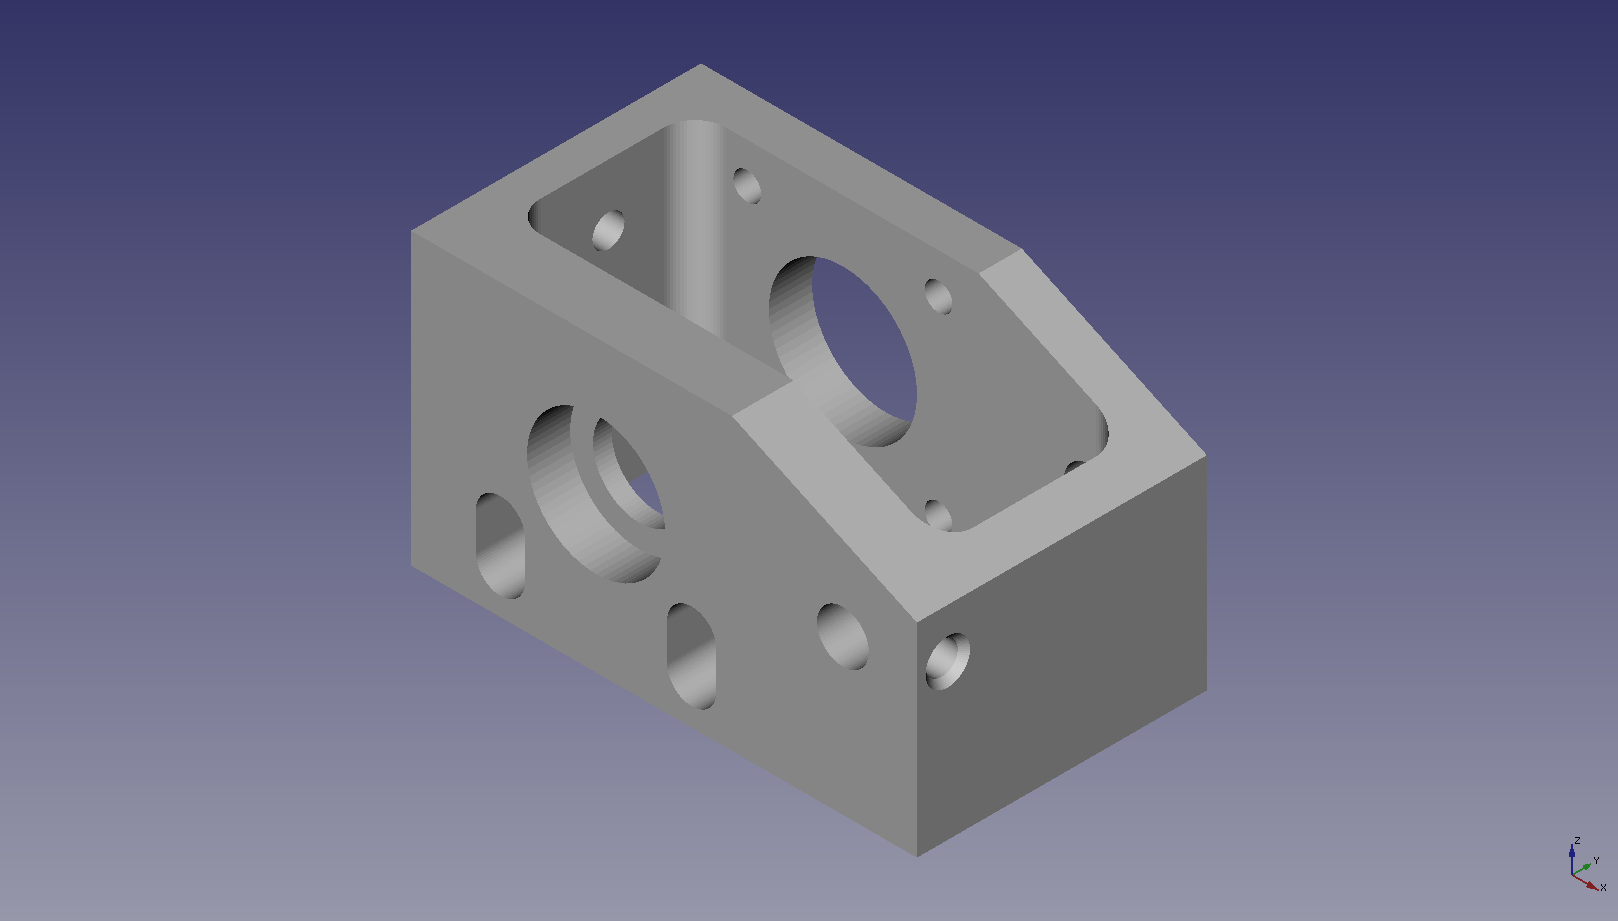
\includegraphics[keepaspectratio=true,angle=0,height=1.0\textheight,width=1.0\textwidth]{STL/lowzleft.stl.png}
\caption{3D Printed Lower Z Left Render}
\label{fig:lowzleftrender}
\end{figure}

\begin{figure}[H]
\centering
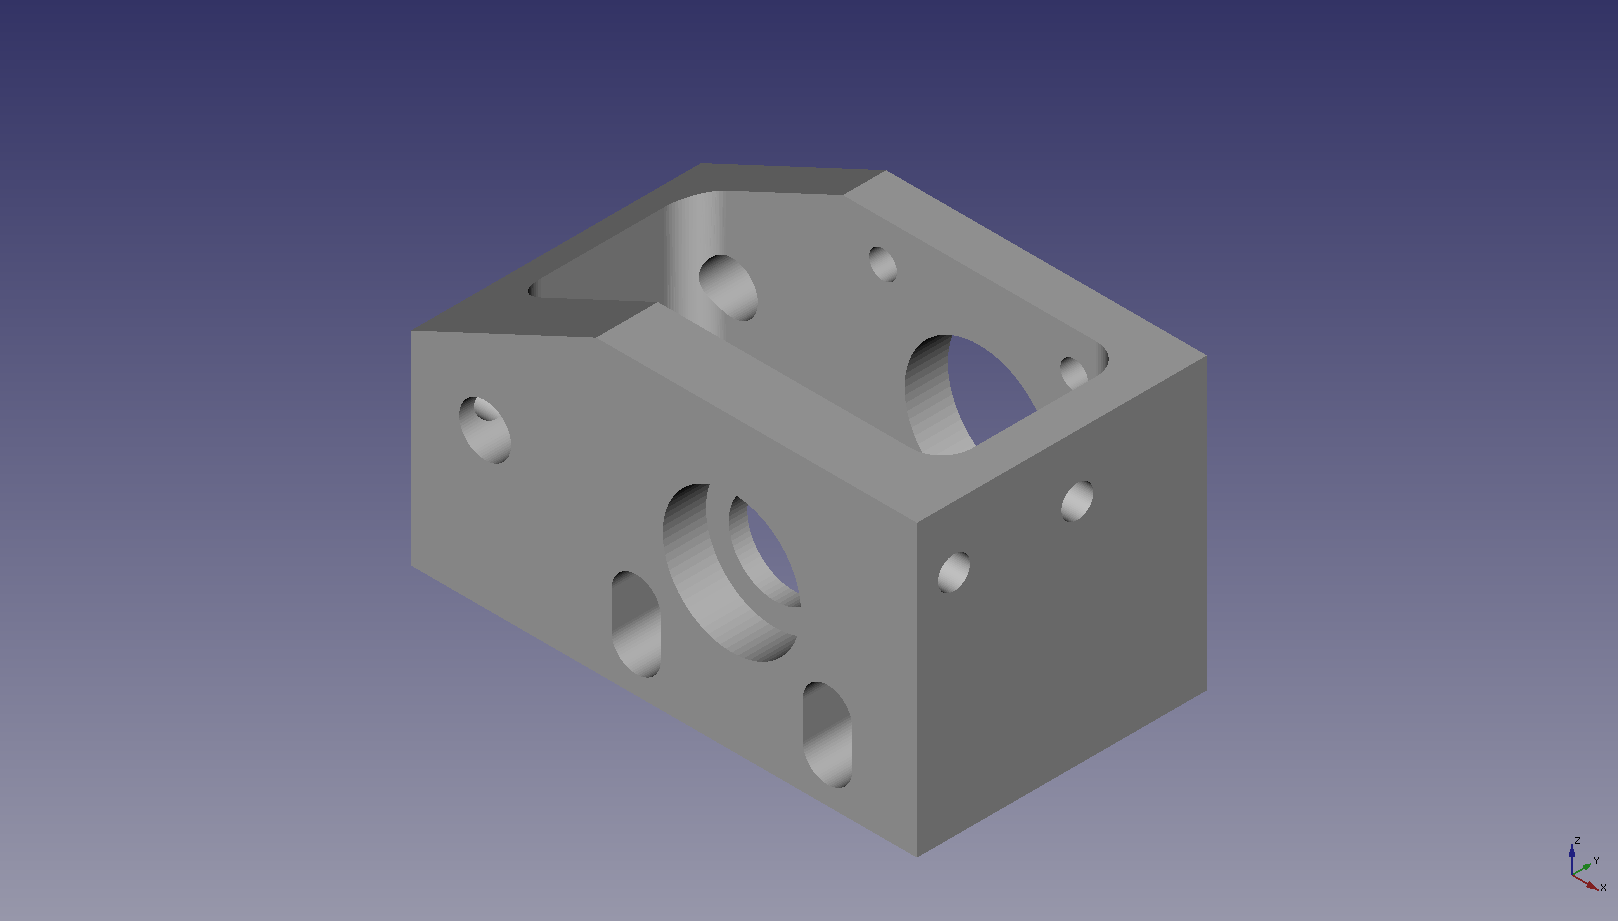
\includegraphics[keepaspectratio=true,angle=0,height=1.0\textheight,width=1.0\textwidth]{STL/lowzright.stl.png}
\caption{3D Printed Lower Z Right Render}
\label{fig:lowzrightrender}
\end{figure}

\begin{figure}[H]
\centering
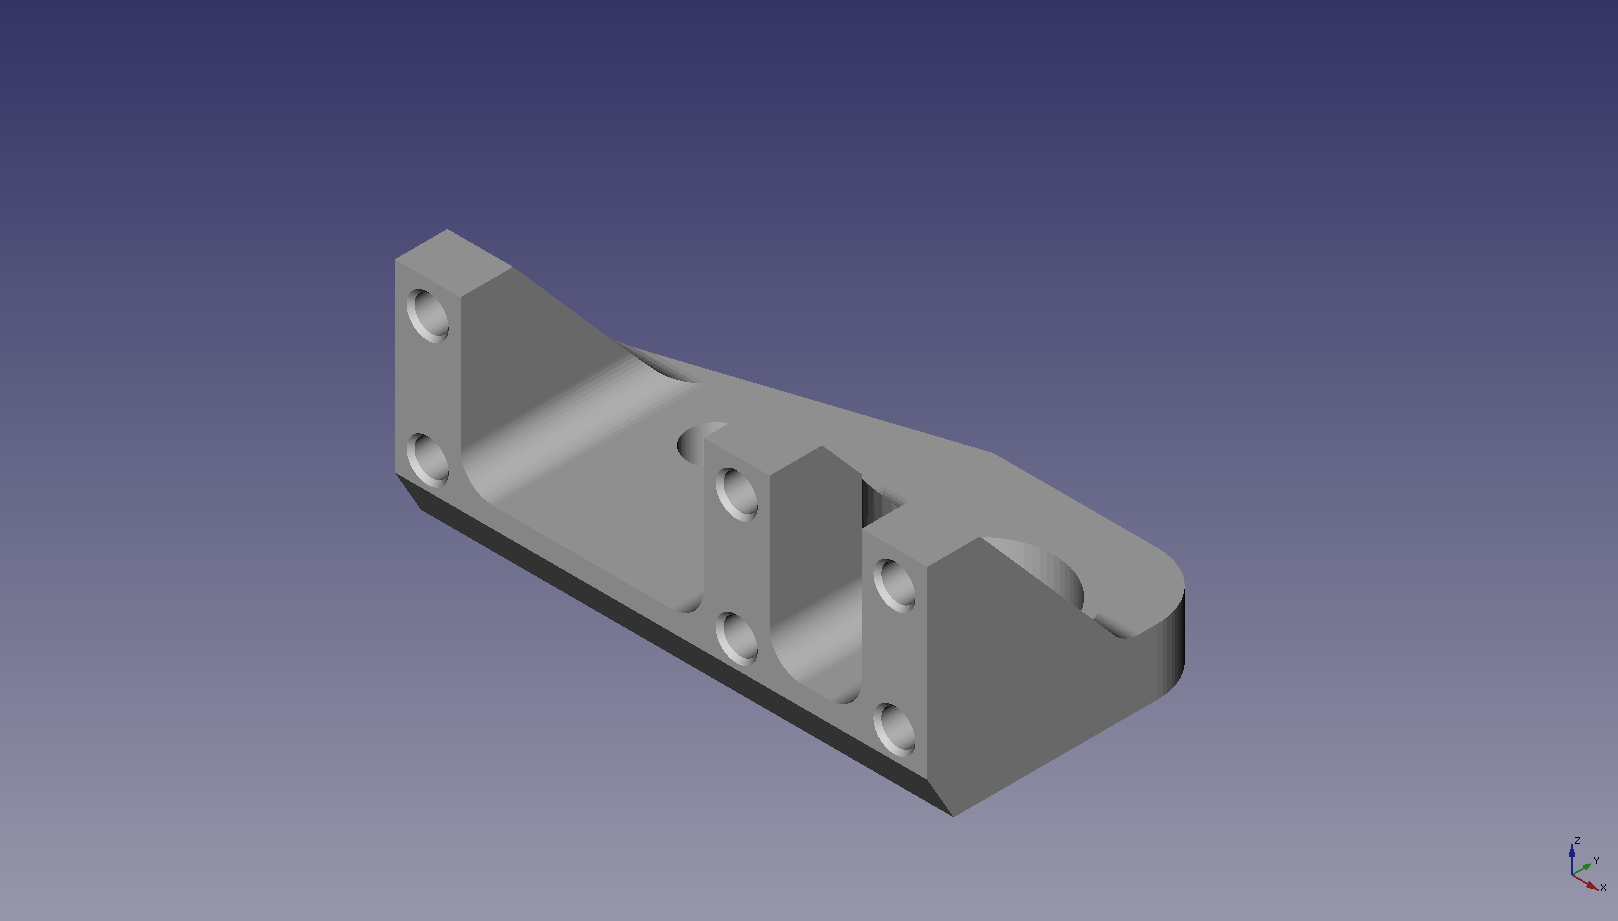
\includegraphics[keepaspectratio=true,angle=0,height=1.0\textheight,width=1.0\textwidth]{STL/upzleft.stl.png}
\caption{3D Printed Upper Z Left Render}
\label{fig:upzleftrender}
\end{figure}

\begin{figure}[H]
\centering
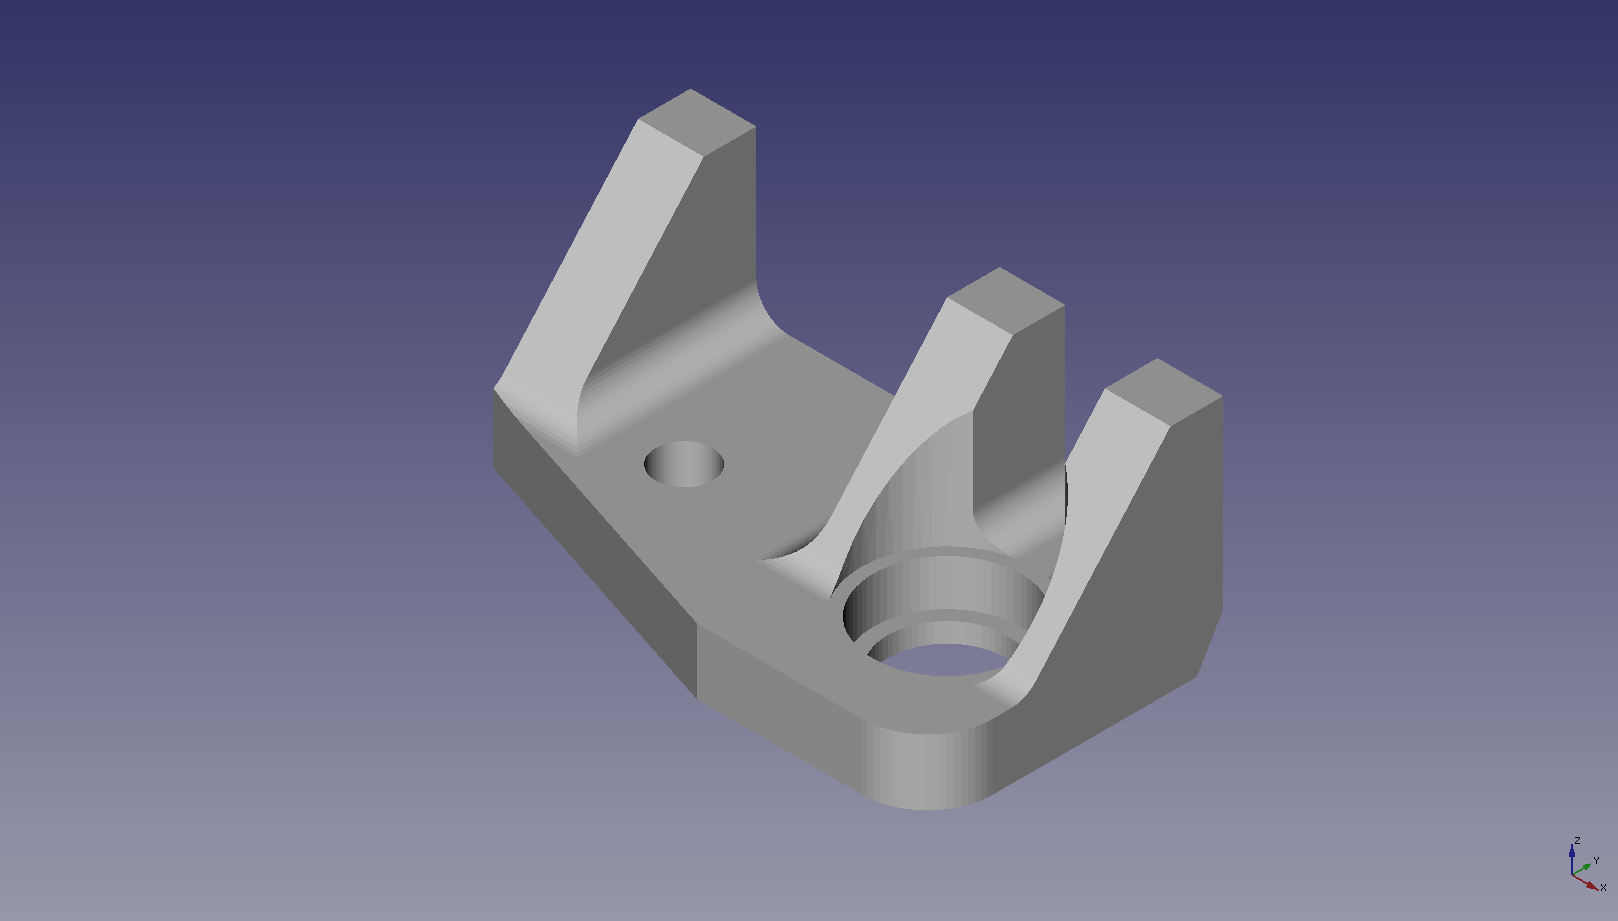
\includegraphics[keepaspectratio=true,angle=0,height=1.0\textheight,width=1.0\textwidth]{STL/upzright.stl.png}
\caption{3D Printed Upper Z Right Render}
\label{fig:upzrightrender}
\end{figure}

\section{Misc}

\begin{figure}[H]
\centering
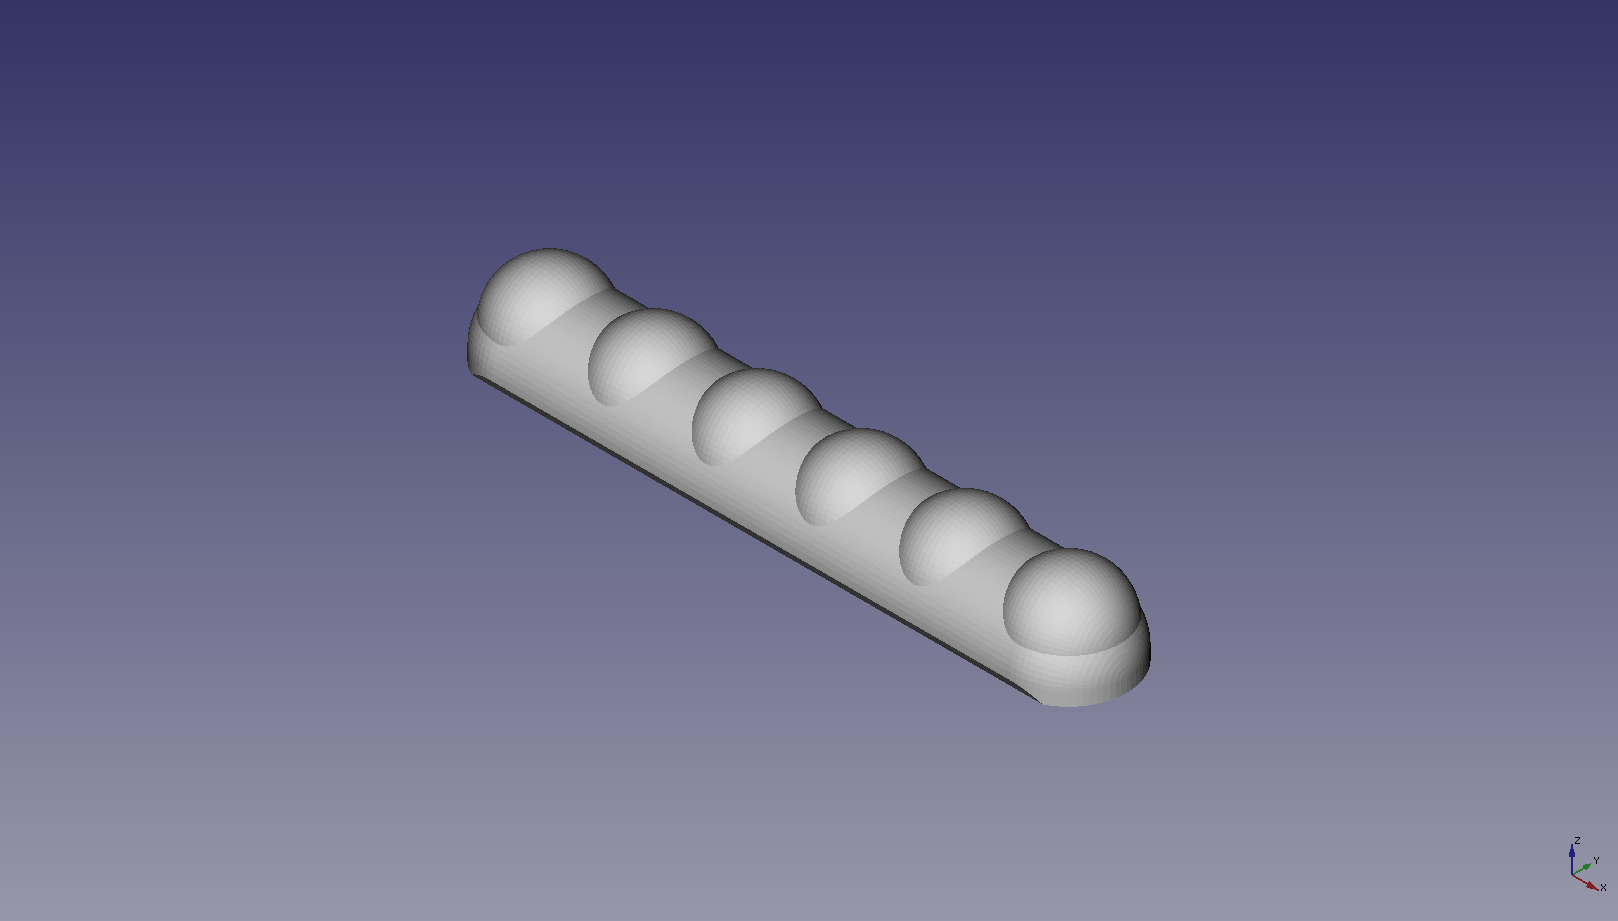
\includegraphics[keepaspectratio=true,angle=0,height=1.0\textheight,width=1.0\textwidth]{STL/handlebar.stl.png}
\caption{3D Printed Handle Bar Render}
\label{fig:handlebarrender}
\end{figure}

\begin{figure}[H]
\centering
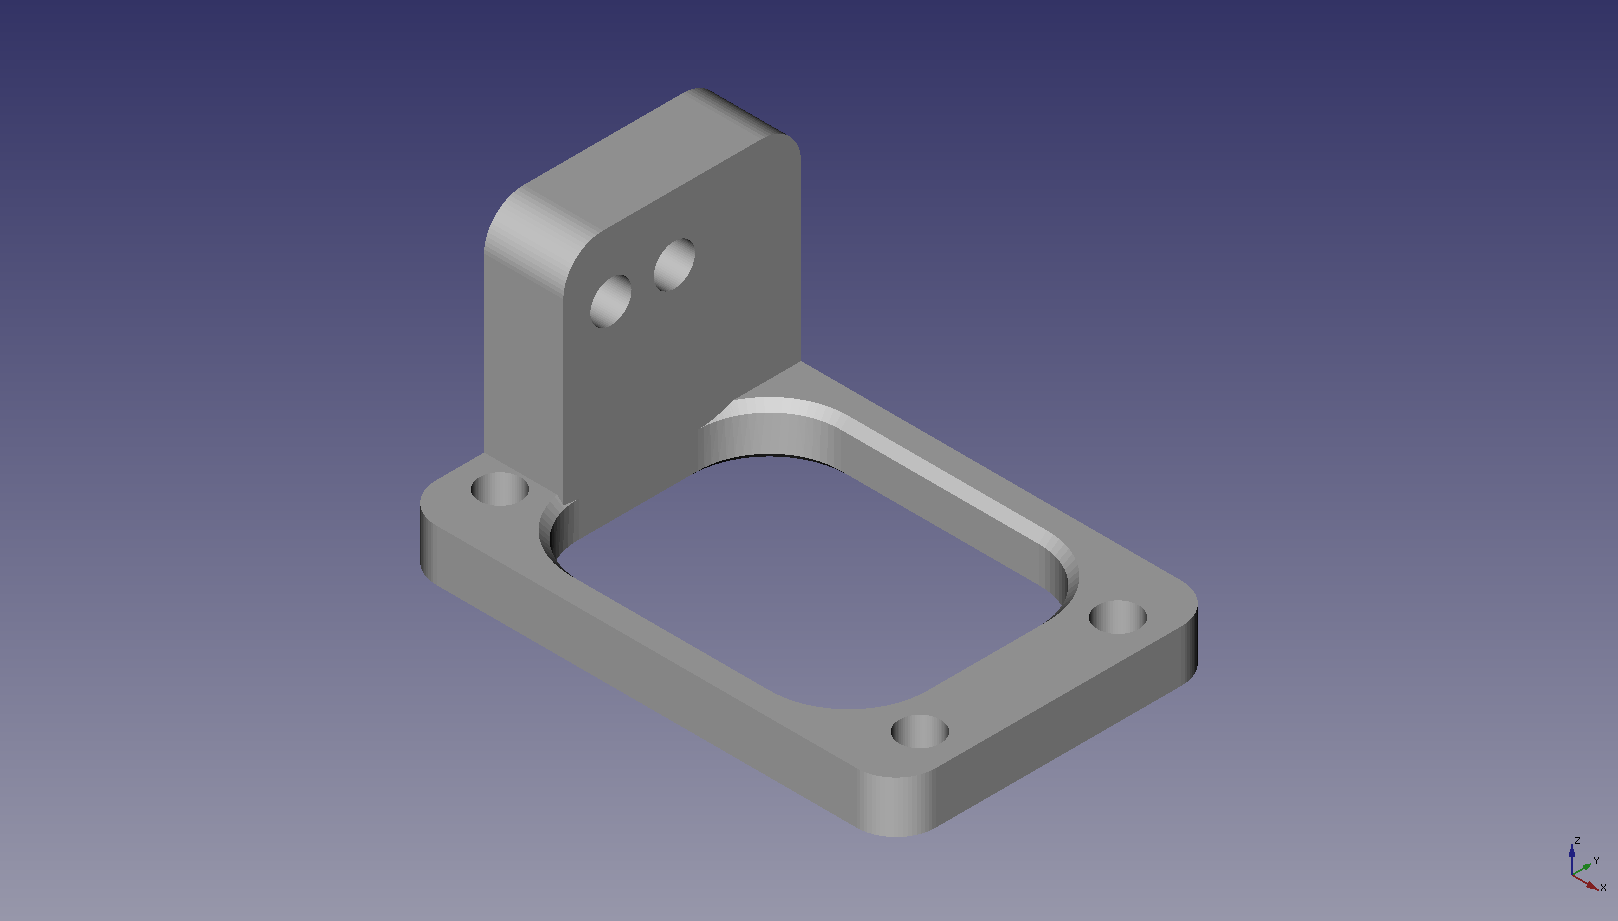
\includegraphics[keepaspectratio=true,angle=0,height=1.0\textheight,width=1.0\textwidth]{STL/reliefmount.stl.png}
\caption{3D Printed Relief Mount Render}
\label{fig:reliefmountrender}
\end{figure}

\begin{figure}[H]
\centering
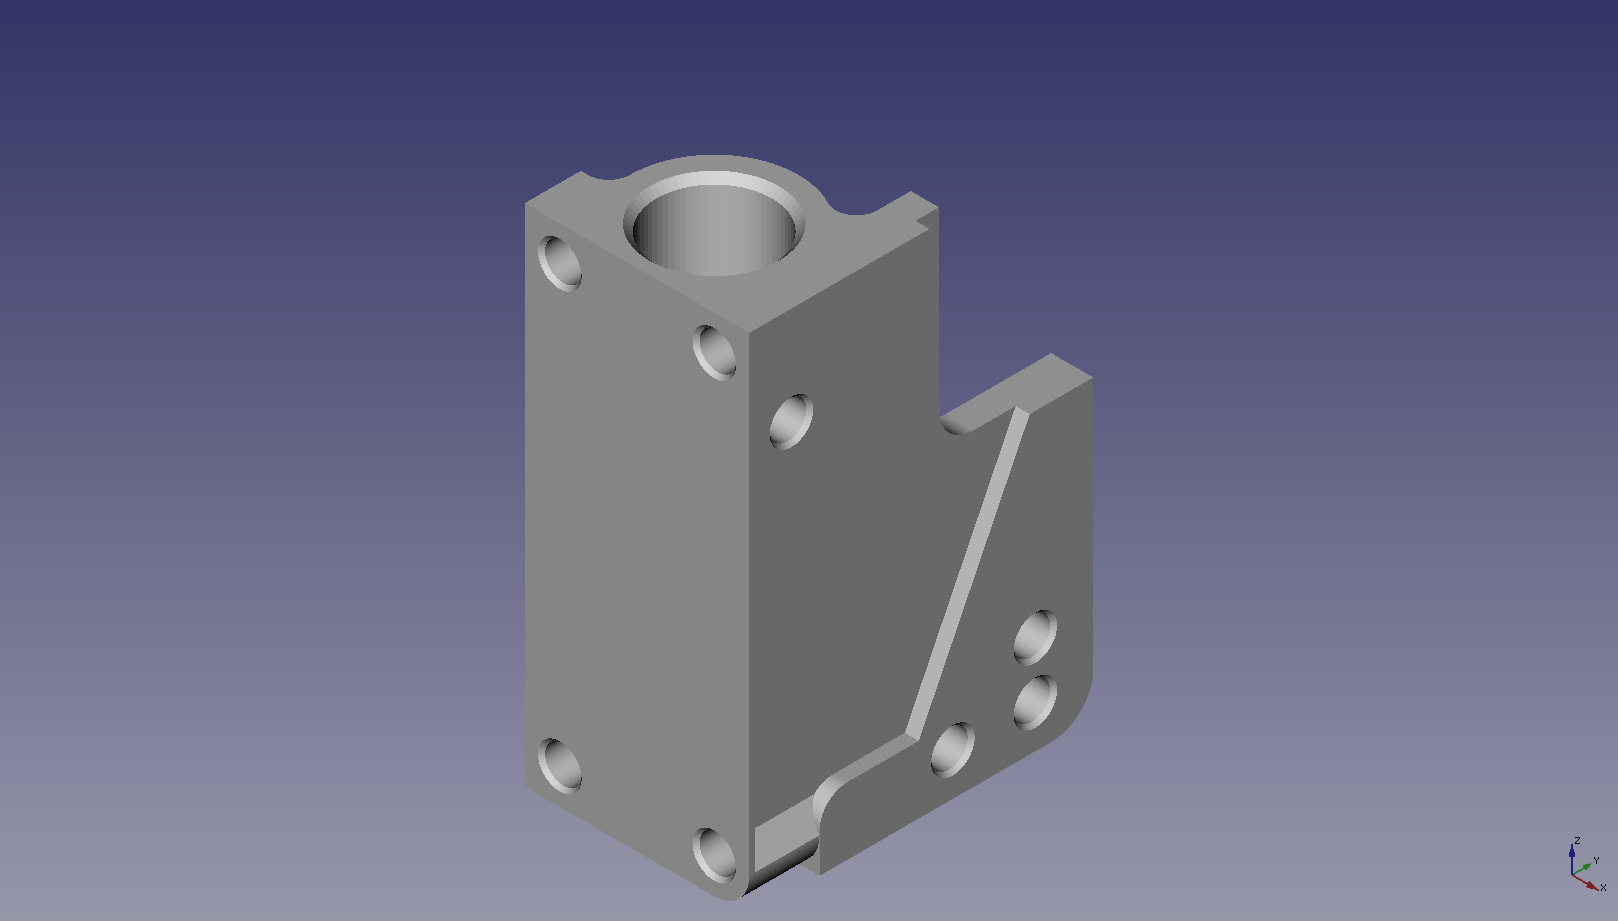
\includegraphics[keepaspectratio=true,angle=0,height=1.0\textheight,width=1.0\textwidth]{STL/upperbearingholder.stl.png}
\caption{3D Printed Upper Bearing Holder Render}
\label{fig:upperbearingholderrender}
\end{figure}

\begin{figure}[H]
\centering
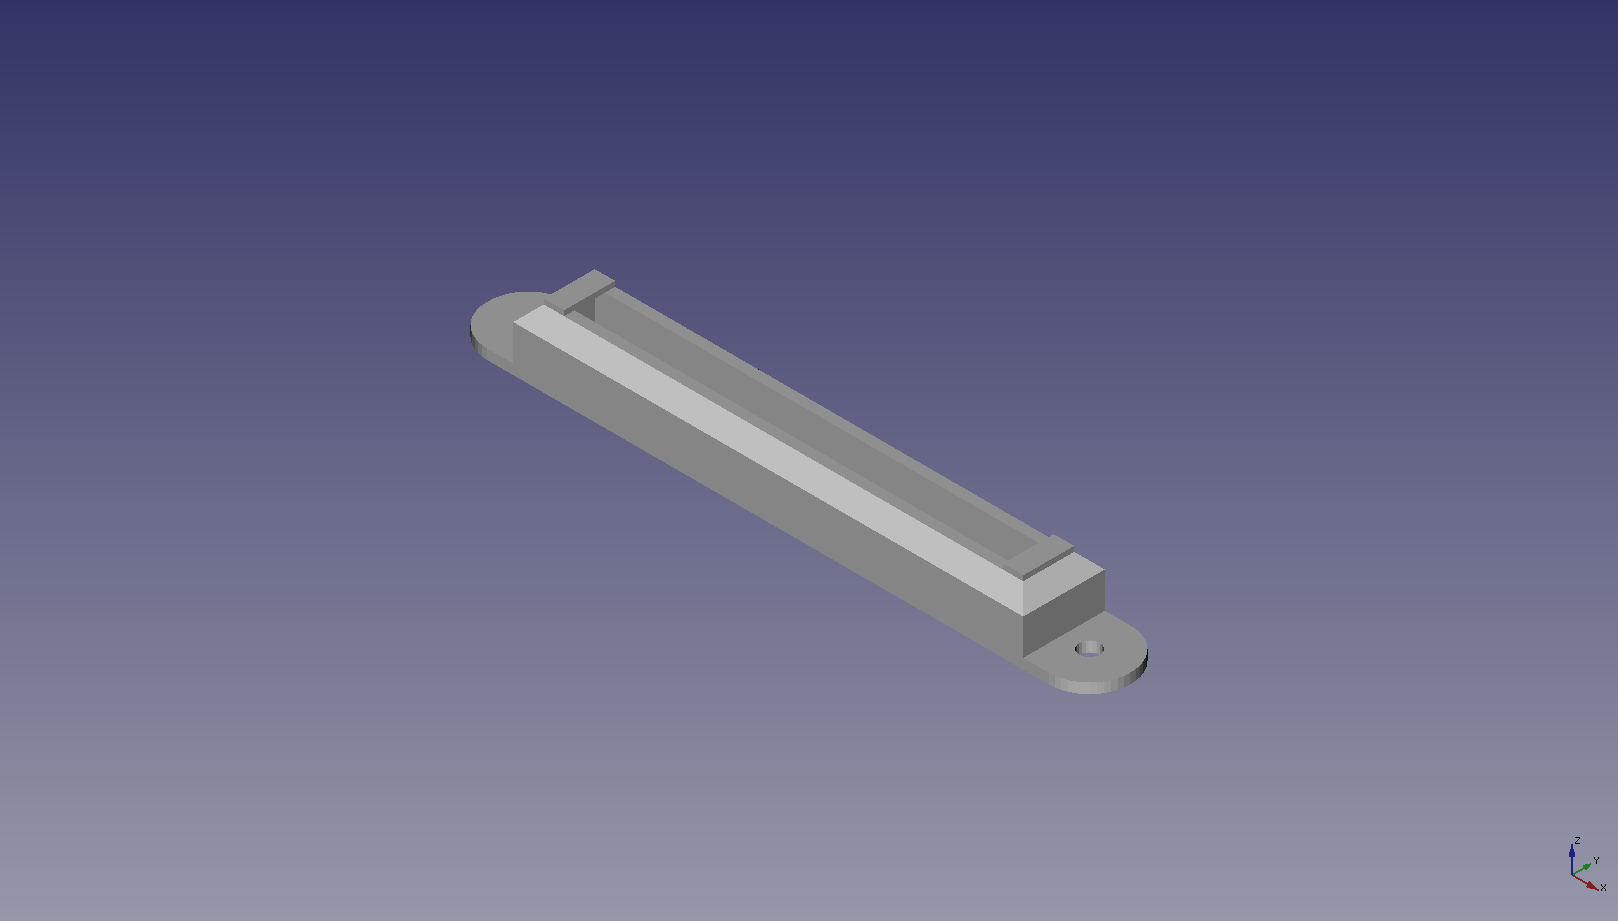
\includegraphics[keepaspectratio=true,angle=0,height=1.0\textheight,width=1.0\textwidth]{STL/wipermount.stl.png}
\caption{3D Printed Wiper Mount Render}
\label{fig:wipermountrender}
\end{figure}

\begin{figure}[H]
\centering
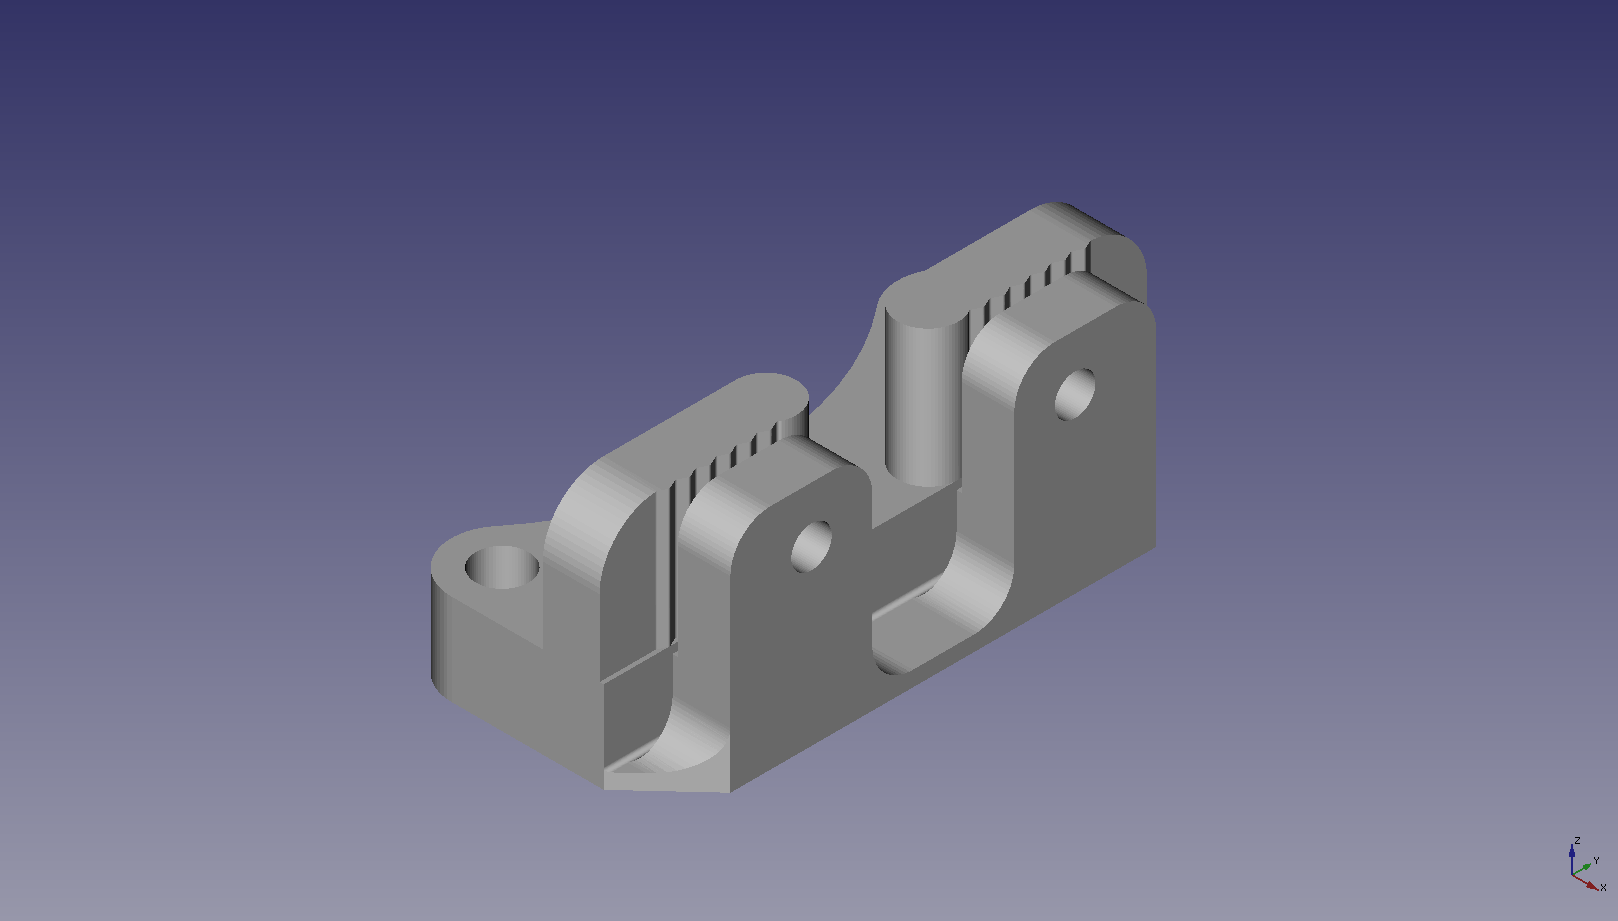
\includegraphics[keepaspectratio=true,angle=0,height=1.0\textheight,width=1.0\textwidth]{STL/beltmount.stl.png}
\caption{3D Printed Belt Mount Render}
\label{fig:beltmountrender}
\end{figure}

